\documentclass[a4paper,10pt]{report}

\usepackage[utf8]{inputenc}
\usepackage[italian]{babel}
\usepackage{amsmath}
\usepackage{amsfonts}
\usepackage{xfrac}
\usepackage{bm}
\usepackage{hyperref}

\usepackage{amsmath}
\usepackage{array}
\usepackage{amstext}
\usepackage{amsthm}
\usepackage{enumitem}
\usepackage{fancyhdr}
\usepackage{eurosym}
\usepackage{amsmath,amssymb}
\usepackage{graphicx}
\usepackage{listings}
\usepackage{lstautogobble}
%\usepackage{color}

%%editing
\usepackage{todonotes}

\lstdefinestyle{customc}{
  belowcaptionskip=1\baselineskip,
  breaklines=true,
  %frame=L,
  xleftmargin=\parindent,
  language=C++,
  showstringspaces=false,
  basicstyle=\footnotesize\ttfamily,
  keywordstyle=\bfseries\color{green!40!black},
  commentstyle=\itshape\color{red},
  identifierstyle=\color{blue},
  stringstyle=\color{orange},
}

\lstset{style=customc}


\hypersetup{
    colorlinks=false,
    pdfborder={0 0 0},
}

\usepackage{listings}
\usepackage{lstautogobble}

\lstset{basicstyle=\ttfamily,
  mathescape=true,
  escapeinside=||,
  autogobble}
  
\setlength{\parindent}{0pt}

\newcommand{\der}[2]{\frac{\partial #1}{\partial #2}}
\newcommand{\dder}[2]{\frac{\partial^2 #1}{\partial #2^2}}
\newcommand{\dmix}[3]{\frac{\partial^2 #1}{\partial #2 \partial #3}}

\theoremstyle{plain}
\newtheorem{theorem}{Teorema}[chapter]
\newtheorem{prop}{Proposizione}[chapter]
\newtheorem{lem}{Lemma}[chapter]
\newtheorem{corollario}{Corollario}[section]

\theoremstyle{definition}
\newtheorem{definition}{Definizione}[chapter]
\newtheorem{notazione}{Notazione}[chapter]

\theoremstyle{remark}
\newtheorem{osservazione}{Osservazione}[chapter]
\newtheorem{esempio}{Esempio}%[chapter]

\begin{document}

\thispagestyle{empty}

	\begin{center}
	 {\large{\textbf{POLITECNICO DI MILANO}\\
             Corso di Laurea Magistrale di Ingegneria Matematica\\
             Facolt\`a di Ingegneria dei Sistemi\\
             }}
	\end{center}

	\vspace{1cm}
	\begin{figure}[htbp]
	\begin{center}
	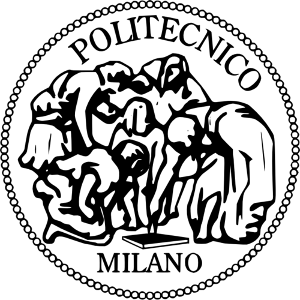
\includegraphics[width=4cm]{img/poli_logo.png}
	\end{center}
	\end{figure}
	
	\vspace{1cm}
	\begin{center}
	{\LARGE{Progetto di Programmazione Avanzata per il Calcolo Scientifico:}}
	\end{center}
	%\color{white}
	\vspace{2cm}
	\begin{center}
	{\LARGE{\textbf{Metodo a elementi finiti per il pricing di opzioni multi-asset con modelli di L\'evy}}}
	\end{center}
	
	%\color{black}
	%\vspace{2.5 cm}
	\begin{table}[hb!]
	\begin{center}
	\begin{tabular}{p{8cm}p{7cm}}
	& \\
  	& \\
  	& {\large Nahuel Foresta, matr. 798775}\\
	& {\large Giorgio G. Re, matr. 799260}\\
	\end{tabular}
	\end{center}
	\end{table}
	\begin{center}
	\vspace{3cm}
	\large{Anno Accademico 2012-2013}
	\end{center}

	\clearpage
	\thispagestyle{empty}
	
	\clearpage

\clearpage
\thispagestyle{plain}
\par\vspace*{.35\textheight}{\raggedleft An approximate answer to the right problem is worth a good deal more than an exact answer to an approximate problem.\par}
\par\vspace{1cm}{\raggedleft John Tukey\par}

\tableofcontents
\listoftodos

\chapter*{Introduzione}

\chapter{Modello di Black \& Scholes}

\section{Introduzione}
In questo capitolo descriviamo i modelli basilari utilizzati per descrivere il mercato finanziario, seguendo le argomentazioni di Merton (1973), trattate in \cite{bjork2009arbitrage}. Consideriamo quindi un mercato finanziario molto semplificato, costituito da un titolo \emph{risk-free} descritto dal processo $B$ e un titolo azionario con valore pari al processo $S$. Definiamo quindi questi due processi.
\begin{definition}
Sia $(\Omega,\mathcal{F},\mu)$ uno spazio misurabile e sia $\mathcal{F}_{t\in [ 0,T ]}$ una filtrazione. Allora, il processo B descrive il valore di un titolo \emph{risk-free} se la sua dinamica \`e del tipo: $$dB(t)=r(t)B(t)dt,$$dove $r$ \`e un qualsiasi processo $\mathcal{F}_t$-adattato.
\end{definition}
La caratteristica pi\`u importante quindi dei processi \emph{risk-free} \`e l'assenza di aleatoriet\`a data da un processo stocastico casuale. Integrando l'equazione precedente, otteniamo: $$B(t)=B(0)\int_0^tr(s)ds.$$ Un caso particolare \`e quello in cui $r$ \`e una costante deterministica, in tal modo $B$ descrive l'andamento di un'obbligazione.\\\\Assumiamo poi che la dinamica di $S$ sia data da: $$dS(t)=S(t)\mu(t,S(t))dt+S(t)\sigma(t,S(t))dW(t),$$ in cui $W_t$ \`e un processo di Wiener (cio\`e, un moto browniano) e $\mu$ e $\sigma$ due funzioni deterministiche. La funzione $\sigma$ \`e detta volatilit\`a del titolo, $\mu$ \`e il tasso di ritorno di $S$.
%\begin{osservazione}
%Osserviamo la differenza fra il tasso di ritorno di un titolo \emph{risk-free} e quello di un titolo rischioso. Il tasso di $B$ \`e: $$\frac{dB(t)}{B(t)dt}=r(t),$$ ovvero totalmente deterministico, mentre quello di $S$ \`e dato da: $$\frac{dS(t)}{S(t)dt}=\mu(t,S(t))+\sigma(t,S(t)) \frac{dW(t)}{dt},$$ oggetto che non \`e osservabile al tempo $t$. Esso \`e infatti costituito da $\mu$ e $\sigma$ che sono entrambi osservabili al tempo $t$, pi\`u un rumore bianco $W(t)$ che \`e del tutto casuale. Quindi, al contrario del titolo \emph{risk-free}, l'azione ha un tasso di ritorno stocastico, anche su una scala infinitesima.
%\end{osservazione}
Passiamo ora a definire il modello di \emph{Black\&Scholes}.
\begin{definition}
Il modello di \emph{Black\&Scholes} consiste di due titoli con le seguenti dinamiche:
\begin{align*}
dB(t)&=rB(t)dt,\\
dS(t)&=\mu S(t)dt+\sigma S(t)dW(t),
\end{align*}
dove $r$, $\mu$ e $\sigma$ sono costanti deterministiche.
\end{definition}

\section{Strumenti derivati e Opzioni}
In questa sezione definiamo gli strumenti derivati e, in particolare le opzioni che abbiamo trattato nel progetto.
\begin{definition}
In finanza, \`e denominato strumento derivato ogni contratto o titolo il cui valore si basa sul valore di mercato di un altro titolo o strumento finanziario, detto sottostante (ad esempio, azioni, valute, tassi di interesse o derivati stessi).
\end{definition}
Definiamo ora il titolo derivato pi\`u semplice, ovvero l'opzione \emph{call} europea.
\begin{definition}
Un'opzione \emph{call} europea con prezzo di esercizio (o \emph{strike price}) $K$ e scadenza $T$ sul sottostante $S$ \`e un contratto finanziario derivato con le seguenti caratteristiche:
\begin{itemize}
\item il titolare del contratto ha, al tempo $T$, il diritto di acquistare un'azione del sottostante al prezzo $K$ dal sottoscrittore del contratto, qualsiasi sia il valore del sottostante $S$ al tempo $T$;
\item il titolare del contratto non ha alcun obbligo di acquistare un'azione del sottostante al tempo $T$;
\item il diritto di acquistare un'azione del sottostante pu\`o essere esercitato solo al tempo $T$.
\end{itemize}
\end{definition}
Osserviamo che la scadenza del contratto e il prezzo d'esercizio sono stabiliti alla stipula del contratto, che per noi sar\`a tipicamente $t=0$.\\Oltre alle opzioni \emph{call} europee, esistono opzioni \emph{put} europee, le quali danno al titolare del contratto il diritto a vendere (anzich\'e comprare) un dato titolo azionario a un prezzo fissato $K$. Le opzioni americane invece (\emph{call} o \emph{put} che siano), permettono di esercitare il diritto all'acquisto o alla vendita dell'azione in ogni istante di tempo $t\in[0,T]$.
\begin{esempio}
Supponiamo di possedere un'opzione \emph{call} con scadenza $T=1$ anno, \emph{strike price} $K=100$\officialeuro$ $ e un sottostante che al tempo $t=0$ vale $S_0=100$\officialeuro. Allora, se fra un anno $S_T=120$\officialeuro$ $, eserciteremo l'opzione, acquistando il sottostante per un prezzo pari a $K=100$\officialeuro$ $, e il sottoscrittore del contratto pagher\`a i rimenenti $S_T-K=20$\officialeuro$ $. Se invece $S_T=80$\officialeuro$ $ non eserciteremo l'opzione, ottenendo un guadagno pari a 0.
\end{esempio}
Osserviamo quindi che il valore a scadenza, cio\`e il \emph{payoff}, dell'opzione dipende soltanto dal valore del sottostante. Definiamo quindi il
%\todo{il payoff non è n processo se T è fisso, in questo caso una v.a}
\emph{payoff} come variabile aleatoria in funzione di $S$.
\begin{definition}
Sia $S$ il processo stocastico che descrive l'andamento di un titolo azionario, allora il \emph{payoff} di un'opzione scritta su $S$ con scadenza $T$ e \emph{strike} $K$ \`e una variabile aleatoria $\mathcal{X}\in\mathcal{F}_T$, e: $$\mathcal{X}=\Phi(S_T).$$
\end{definition}
Per esempio, il \emph{payoff} delle opzioni call e put europee \`e:
\begin{align*}
\Phi(S_T)&=\max(S_T-K,0),\\
\Phi(S_T)&=\max(K-S_T,0).
\end{align*}
La domanda che ci poniamo ora \`e la seguente: qual \`e il prezzo equo di un'opzione? Ovvero, quanto occorre pagare oggi per avere il diritto ma non l'obbligo di acquistare al tempo $T$ un'azione a un prezzo fissato $K$?

\section{L'equazione di \emph{Black\&Scholes}}
Vi sono molti modi per ricavare l'equazione di \emph{Black\&Scholes}: presentiamo qui il modo pi\`u semplice e veloce.\\\\Prima di ricavare l'equazione spendiamo qualche riga per descrivere il concetto di neutralit\`a al rischio in finanza. Un operatore economico si dice neutrale al rischio quando le sue preferenze lo rendono indifferente al compiere un'azione il cui risultato \`e una quantit\`a aleatoria, oppure compiere un'azione il cui risultato \`e il valore atteso della quantit\`a aleatoria stessa.\\Per esempio, per un soggetto neutrale al rischio sono indifferenti le seguenti situazioni:
\begin{itemize}
\item avere $1$\officialeuro$ $ con probabilit\`a 1;
\item giocare a una lotteria in cui il soggetto pu\`o ricevere $2$\officialeuro$ $ con probabilit\`a $\sfrac{1}{2}$ o $0$\officialeuro$ $ con probabilit\`a $\sfrac{1}{2}$.
\end{itemize}
Nel primo caso infatti, egli ottiene sempre $1$\officialeuro$ $, nel secondo ottiene in media $1$\officialeuro$ $. Perci\`o per un soggetto neutrale al rischio queste situazioni sono indifferenti.\\Quando ci occupiamo di \emph{pricing} di derivati, ci poniamo sempre nell'ipotesi di neutralit\`a al rischio. In particolare,
\begin{enumerate}
\item assumiamo che il termine di deriva $\mu$ del modello $S$ sia pari al tasso di interesse \emph{risk-free} $r$, cio\`e poniamo: $$dS(t)=rS(t)dt+\sigma S(t)dW(t);$$
\item calcoliamo il valore atteso del \emph{payoff}, cio\`e $\mathbb{E}\left[\Phi(S_T)|\mathcal{F}_t\right]$;
\item scontiamo il valore atteso del \emph{payoff} con il tasso di interesse $r$.
\end{enumerate}
Sia quindi $C:\mathbb{R}^+\times[0,T]\rightarrow\mathbb{R}^+$, $C=C(S(t),t)$ il processo stocastico che descrive il valore di un'opzione. In particolare,
%\todo{forse ci vuole il condizionamento}
se consideriamo una \emph{call} europea,
$$C(S,t)=e^{(-r(T-t))}\mathbb{E}\left[\max(S_T-K,0)|\mathcal{F}_t\right].$$
Data la dinamica di $S$, se applichiamo a questa quantit\`a il Lemma di It$\hat{o}$, otteniamo la seguente equazione: $$dC(S,t)=\left(\der{C}{t}+r S \der{C}{S} +\frac{1}{2}S^2\dder{C}{S}\right)dt+\sigma S \der{C}{S}dW(t).$$
Dall'altro lato per\`o, per la \emph{risk-neutrality}, la deriva di $C$, come quella di ogni titolo finanziario, dovr\`a essere pari a $rC$, quindi:$$\der{C}{t}+r S \der{C}{S} +\frac{1}{2}S^2\dder{C}{S}=rC.$$
Riassumendo, posti $C=C(S,t)$ e $P=P(S,t)$ i processi che descrivono il prezzo di opzioni \emph{call} e \emph{put}, otteniamo le seguenti equazioni alle derivate parziali con le rispettive condizioni finali e condizioni al bordo:
\begin{equation}
\begin{cases}
\displaystyle
\der{C}{t}+r S \der{C}{S} +\frac{1}{2}S^2\dder{C}{S}=rC,\\
C(S,T)=\max(S_T-K,0),\\
C(0,t)=0,\qquad\quad\qquad\forall t\in[0,T],\\
\lim\limits_{S\to\infty}C(S,t)=\infty,\qquad\forall t\in[0,T],
\end{cases}
\label{callbs1d}
\end{equation}
e
\begin{equation}
\begin{cases}
\displaystyle
\der{P}{t}+r S \der{P}{S} +\frac{1}{2}P^2\dder{P}{S}=rP,\\
P(S,T)=\max(K-S_T,0),\\
P(0,t)=K,\qquad\qquad\forall t\in[0,T]\\
\lim\limits_{S\to\infty}P(S,t)=0,\qquad\forall t\in[0,T].
\end{cases}
\label{putbs1d}
\end{equation}
Come possiamo osservare, si tratta di equazioni paraboliche \emph{backward} con dato finale. Il prezzo dell'opzione sar\`a dato dalla soluzione C o P, valutate in $S_t=S_0$, ovvero il valore dell'azione oggi, e in $t=0$.

\section{Opzioni Basket}
Un altro tipo di opzioni scambiate sui mercati finanziari sono le opzioni basket, il cui \emph{payoff} dipende cio\`e da due o pi\`u sottostanti. In particolare, in questo progetto ci siamo concentrati sul \emph{pricing} di opzioni basket 2D, con i seguenti valori finali: $$C(S_1, S_2, T)=\max(S_{1,T}+S_{2,T}-K,0)$$ per la \emph{call} e: $$P(S_1, S_2, T)=\max(K-S_{1,T}-S_{2,T},0)$$ per la \emph{put}, dove $S_{1,T}$ e $S_{2,T}$ sono i valori al tempo $T$ dei due sottostanti $S_1$ e $S_2$.\\L'equazione che si ottiene con procedimenti analoghi a quelli mostrati nella sezione precedente \`e la seguente:
\begin{equation}
\der{C}{t}+rS_1\der{C}{S_1}+rS_2\der{C}{S_2}+\frac{\sigma^2_1}{2}S_1^2\dder{C}{S_1}+\frac{\sigma^2_2}{2}S_2^2\dder{C}{S_2}+\rho\sigma_1\sigma_2\dmix{C}{S_1}{S_2}=rC,
\label{pde2d}
\end{equation}
in cui $C:\mathbb{R}^+\times\mathbb{R}^+\times[0,T]\rightarrow\mathbb{R}^+$, $C=C(S_1(t), S_2(t),t)$, $\sigma_1$ e $\sigma_2$ sono le volatilit\`a dei due sottostanti e $\rho$ \`e il coefficiente di correlazione fra $S_1$ e $S_2$.

\section{Opzioni Americane: il problema con frontiera libera}
Le opzioni americane differiscono dalle europee poich\'e consentono di esercitare l'opzione non solo in $T$, bens\`i in qualsiasi istante di tempo dalla stipula del contratto alla sua scadenza. Quindi, proprio perch\'e danno al titolare del contratto dei diritti aggiuntivi, \`e facile capire che vale la seguente relazione: $$V^{Am}\geq V^{Eu},$$ ovvero il valore di un'opzione americana \`e sempre superiore al valore dell'europea corrispondente. In particolare, il valore dell'opzione americana \`e sempre pari o superiore al valore del \emph{payoff}. L'opzione europea infatti, pu\`o avere un valore inferiore al \emph{payoff}, ma questo non pu\`o succedere per le americane. Infatti, se cos\`i non fosse, potremmo acquistare un'azione e una \emph{put} su questa azione ed esercitare immediatamente\todo{Spieghiamo meglio o ce ne strafottiamo?}, ottenendo un guadagno certo senza correre alcun rischio. Per questo valgono i seguenti vincoli:
\begin{align}
C^{Am}(S,t)&\geq \max(S_T-K,0)\qquad\forall t\in[0,T],\\
P^{Am}(S,t)&\geq \max(K-S_T,0)\qquad\forall t\in[0,T].
\label{putbound}
\end{align}
\begin{figure}[h!]
\begin{center}
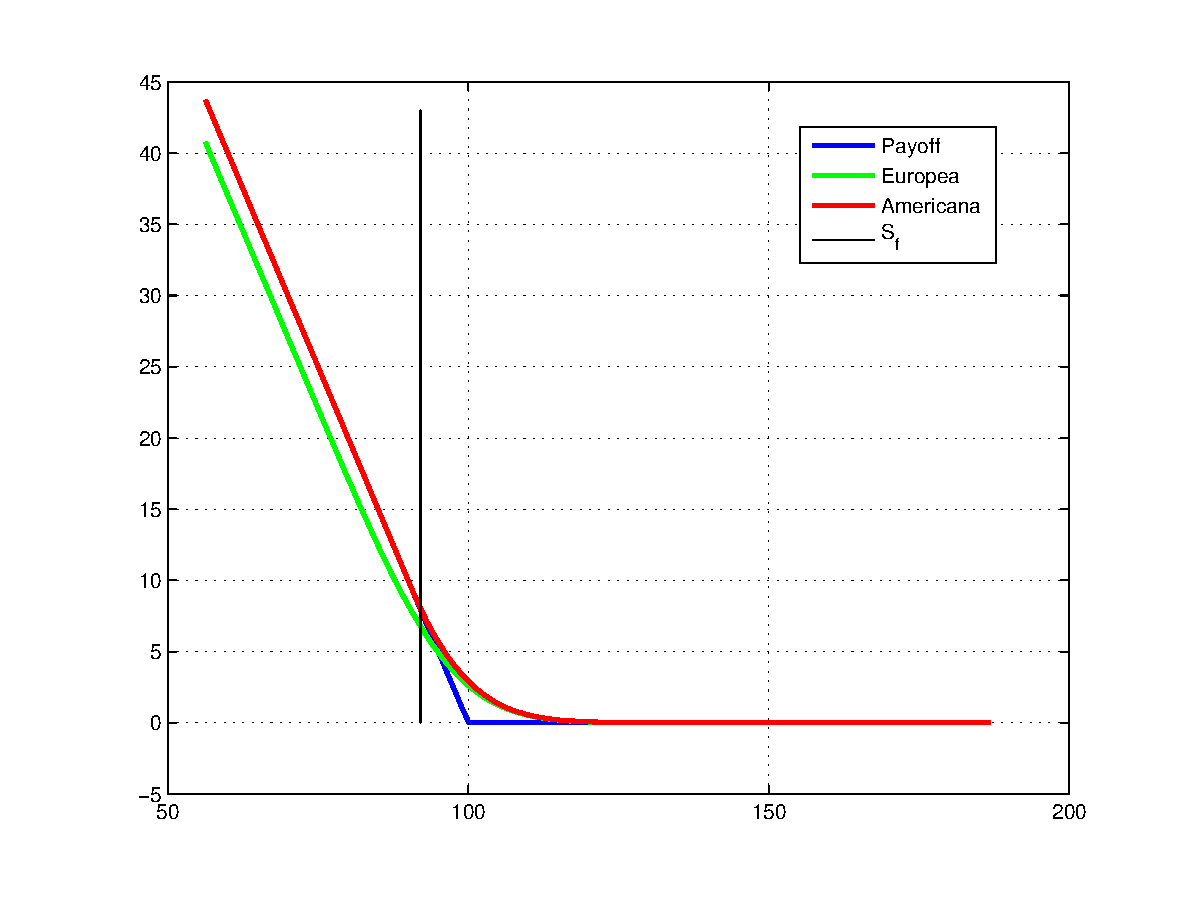
\includegraphics[width=12cm]{img/putam.eps}
\caption{Opzioni Americane vs. Opzione Europee}
\label{putamfig}
\end{center}
\end{figure}
Consideriamo ora il comportamento della \emph{put} nella parte sinistra del grafico riportato in figura \ref{putamfig}. Senza la possibilt\`a di esercizio anticipato, $P^{Eu}<K-S$, ma per la disuguaglianza \ref{putbound}, $P^{Am}=K-S$. Nella parte destra della curva, invece, vale $P^{Am}\geq \max(K-S,0)$. Quindi, per la continuit\`a e la monotonia di $P^{Am}$, la curva dovr\`a toccare il \emph{payoff} in un punto $S_f(t)$, $0<S_f(t)<K$. Questo punto \`e definito da:
\begin{align*}
P^{Am}(S,t)&>\max(K-S,0)\qquad S>S_f(t),\\
P^{Am}(S,t)&=K-S\qquad\qquad\quad S<S_f(t).
\end{align*}
Quindi, $\forall t\in[0,T]$, dobbiamo determinare il punto $S_f(t)$, attraverso il quale passa la retta che separa l'area in cui $P^{Am}=$\emph{payoff} da qualla in cui $P^{Am}>$\emph{payoff}. Poich\'e a priori questa frontiera \`e ignota, questo problema \`e detto ``a frontiera libera".\\\\Per le \emph{call} americane la situazione \`e differente, poich\'e $C^{Eu}\geq \max(S_T-K,0)$\footnote{Questa relazione si calcola immediatamente sfruttando alcune semplici relazioni che legano $C$, $S$ e $K$. In particolare, nel qual caso: $C^{Am}\geq C^{Eu} \geq S-Ke^{-r(T-t)} > S-K$}. Perci\`o il prezzo di una \emph{call} americana \`e identico a quello di un'europea e in questo caso non si pone il problema con frontiera libera.\\\\Formalmente, l'equazione differenziale che occorre risolvere per trovare il prezzo di una \emph{put} americana \`e la seguente:
\begin{equation}
\begin{cases}
\displaystyle
\der{P}{t}+r S \der{P}{S} +\frac{1}{2}P^2\dder{P}{S}\leq rP,\\
P(S,t)\geq \max(K-S_T,0),\\
P(S,T)=\max(K-S_T,0),\\
P(0,t)=K,\qquad\qquad\forall t\in[0,T]\\
\lim\limits_{S\to\infty}P(S,t)=0,\qquad\forall t\in[0,T].
\end{cases}
\label{putam1d}
\end{equation}
%nel caso monodimensionale, occorre aggiungere ai problemi \ref{callbs1d} e \ref{putbs1d} rispettivamente i seguenti vincoli: $$C(S,t)\geq \max(S_t-K,0), \qquad\forall t\in[0,T],$$ e $$P(S,t)\geq \max(K-S_t,0),\qquad\forall t\in[0,T].$$

\section{Difetti del modello di \emph{Black\&Scholes}}
Il modello di \emph{Black\&Scholes}, nonostante sia molto utilizzato in finanza, presenta alcuni problemi e pu\`o essere pericoloso utilizzarlo per valutare strumenti derivati. In particolare, empiricamente, si evidenziano le seguenti problematiche:
\begin{itemize}
\item il valore di $S$ pu\`o essere discontinuo, ovvero \`e possibile che il sottostante presenti dei "salti";
\item le code della distribuzione dei log-rendimenti dovrebbero essere normali, ma non lo sono: i valori delle code sono infatti pi\`u probabili di quanto ipotizzato dal modello, inoltre le code non sono simmetriche poich\'e presentano un'asimmetria verso i rendimenti negativi;
\item i log-rendimenti inoltre non hanno distribuzioni indipendenti: nelle serie storiche si osservano infatti i cosiddetti \emph{cluster}, ovvero periodi in cui la volatilit\`a \`e alta e rimane alta oppure periodi con una volatilit\`a che rimane per ridotta per lungo tempo;
\item in figura \ref{smile} \`e rappresentato il grafico volatilit\`a vs. \emph{moneyness}\footnote{La \emph{moneyness} di un'opzione \`e il rapporto fra prezzo del sottostante in $t=0$ e \emph{Strike}, ovvero $\sfrac{S_0}{K}$.}. In esso possiamo osservare che il valore della volatilit\`a non rimane costante al variare dei prezzi di esercizio, bens\`i presenta una forma convessa. Questo fenomeno \`e noto come \emph{smile} di volatilit\`a.\todo{Qui, 1. \`e da mettere il disegno? 2. Visto che merton e kou non risolvono questo problema, conviene parlare dello smile o lo saltiamo?}
\end{itemize}
\begin{figure}[htbp!]
\begin{center}
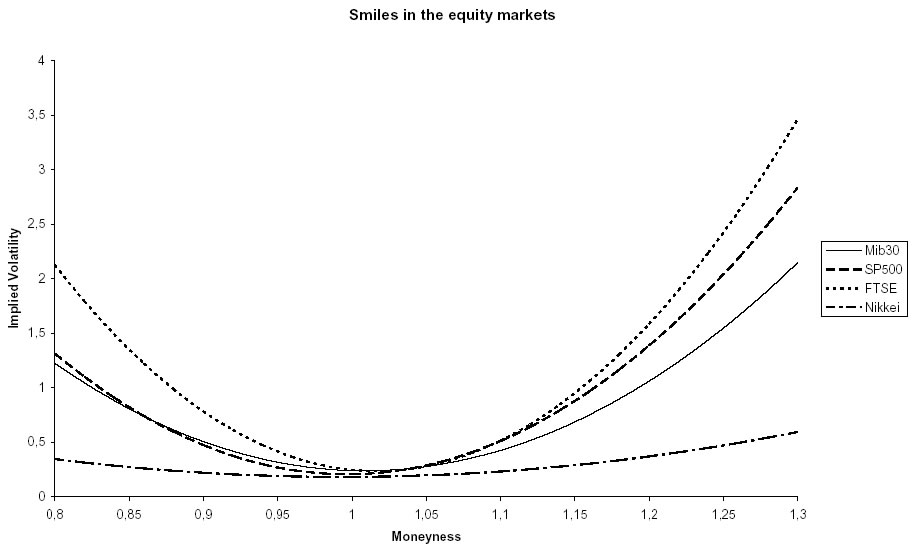
\includegraphics[width=11cm]{img/smile.jpg}
\caption{\emph{Smile} di volatilit\`a}
\label{smile}
\end{center}
\end{figure}
Nel prossimo capitolo introdurremo una classe pi\`u ampia di processi stocastici, cio\`e i processi di L\'evy, e descriveremo dei modelli che permettono di risolvere alcuni dei problemi sopra descritti. Questi modelli danno luogo a equazioni simili a quella di \emph{Black\&Scholes} (PDE) con l'aggiunta per\`o di un termine integrale, per questo le chiameremo Equazioni Integro-Differenziali alle Derivate Parziali (PIDE).

\chapter{Processi di L\'evy e Modelli di Kou e Merton}
\section{Introduzione}
In questo secondo capitolo introduciamo i processi di L\'evy, una classe pi\`u ampia di processi stocastici che permettono di descrivere con pi\`u accuratezza il comportamento di un titolo azionario. Elenchiamo ora alcune definizioni e un teorema che ci permettono di definire i nuovi modelli.
\begin{definition}
Sia $(\Omega, \mathcal{F}, \mu)$ uno spazio misurabile e sia $\mathcal{F}_{t\in[0,T]}$ una filtrazione. Sia $X_t$ un processo stocastico \emph{cadlag}\footnote{Ricordiamo che un processo \`e detto \emph{cadlag} se ha traiettorie continue a destra e limitate a sinistra.}, allora $X_t$ \`e di L\'evy se:
\begin{enumerate}
\item $X_0=0$,
\item ha incrementi indipendenti,
\item ha incrementi stazionari,
\item c'\`e continuit\`a stocastica, ovvero: $$\forall \varepsilon >0,\qquad\lim_{h\to0}\mathbb{P}(|X_{t+h}-X_t|\geq\varepsilon)=0.$$
\end{enumerate}
\end{definition}
\begin{definition}
Sia $X_t$ un L\'evy, allora poniamo $$\nu(A)=\mathbb{E}(\#\{t\in[0,1]: \Delta X_t\neq0, \Delta X_t\in A\}),$$ $\forall A\in \mathcal{B}$, e chiamiamo $\nu(A)$ la misura di L\'evy di $X_t$.
\end{definition}
\begin{definition}
Sia $X_t$ un processo di L\'evy, allora $X_t$ \`e un \emph{Compound Poisson} di intensit\`a $\lambda$ e distribuzione di salti $f$ se: $$X_t=\sum_{i=1}^{N_t}Y_i,$$ dove $N_t\sim$\emph{Poisson}$(\lambda)$ e $Y_i\sim f$, $Y_i$ i.i.d. $\forall i$.
\end{definition}
\begin{theorem}
Decomposizione di L\'evy-It$\hat{o}$ per processi ad attività finita.\\Sia $X_t$ un processo di L\'evy con misura $\nu$ finita, allora esistono due costanti $\gamma$ e $\sigma$ tali che:$$X_t=\gamma t+\sigma W_t+X^C_t,$$ dove $W_t$ \`e un moto browniano e $X^C_t$ un \emph{Compound Poisson}.
\end{theorem}
Perci\`o un processo di L\'evy \`e determinato univocamente dalla sua tripletta caratteristica $(\gamma, \sigma, \nu)$.
\section{Modelli di Merton e Kou}
Passiamo ora a definire i modelli di Merton e Kou. In entrambi questi modelli il prezzo dell'azione \`e descritto dalla seguente equazione:
\begin{equation}
S_t=S_0e^{rt+X_t},
\label{explevy}
\end{equation}
dove $r$ \`e il tasso di interesse e $X_t$ \`e un L\'evy ad attivit\`a finita, ovvero $$X_t=\gamma t+\sigma W_t+\sum_{i=1}^{N_t}Y_i.$$Nel modello di Merton, $Y_i\sim\mathcal{N}(\mu, \delta^2)$, e la misura di L\'evy \`e data da:
\begin{equation}
\nu(x)=\frac{\lambda}{\sqrt{2\pi\delta^2}}exp\left\{-\frac{(x-\mu)^2}{2\delta^2}\right\},
\label{merton}
\end{equation}
in cui $\lambda$ \`e l'intensit\`a del \emph{Poisson}.\\Nel modello di Kou invece, le $Y_i$ sono delle esponenziali con parametri diversi per salti positivi e negativi. In particolare, $$\nu(x)=p\lambda\lambda_+e^{\lambda_+x}\mathcal{I}_{x>0}+(1-p)\lambda\lambda_-e^{-\lambda_-x}\mathcal{I}_{x<0},$$dove $p$ \`e la probabilit\`a di salti positivi, $\lambda$ \`e il solito parametro del \emph{Poisson}, $\lambda_+$ e $\lambda_-$ sono invece le intensit\`a dei salti positivi e negativi.
\section{\emph{Pricing} con modelli Exponential L\'evy}
Riportiamo ora un risultato che permette di individuare un'equazione differenziale che permetta di risolvere il problema di \emph{pricing} descritto nel capitolo precedente.
\begin{theorem}
Sia $S_t$ nella forma \ref{explevy} con l'ipotesi: $$\int_{|x|>1} e^{2x}\nu(dx)<\infty.$$ Sia $C:\mathbb{R}^+\times[0,T]\rightarrow\mathbb{R}^+$, $C=C(S_t,t)$ nella forma: $$C(S_t,t)=e^{-r(T-t)}\mathbb{E}(\Phi(S_t)),$$ dove $\Phi$ \`e un \emph{payoff Lipshitz} che dipende dall'unico sottostante $S_t$. Allora $C$ soddisfa l'equazione:
\begin{multline}
\der{C}{t}+\frac{\sigma^2}{2}S^2\dder{C}{S}+r\der{C}{S}-rC+\\+ \int_\mathbb{R}\left(C(t,Se^y)-C(t,S)-S(e^y-1)\der{C}{S}(t,S)\right)\nu(dy)=0.
\end{multline}
\end{theorem}
Per quanto riguarda opzioni su due \emph{asset}, nell'ipotesi che le parti di salto dei due sottostanti siano indipendenti fra di loro, l'equazione \ref{pde2d} diventa:
\begin{multline}
\der{C}{t}+rS_1\der{C}{S_1}+rS_2\der{C}{S_2}+\frac{\sigma^2_1}{2}S_1^2\dder{C}{S_1}+\frac{\sigma^2_2}{2}S_2^2\dder{C}{S_2}+\rho\sigma_1\sigma_2S_1S_2\dmix{C}{S_1}{S_2}-rC\\+\int_\mathbb{R}\left(C(t,S_1e^y,S_2)-C(t,S_1,S_2)-S_1(e^y-1)\der{C}{S_1}(t,S_1,S_2)\right)\nu_1(dy)\\+\int_\mathbb{R}\left(C(t,S_1,S_2e^y)-C(t,S_1,S_2)-S_2(e^y-1)\der{C}{S_2}(t,S_1,S_2)\right)\nu_2(dy)=0,
\label{pide2d}
\end{multline}
dove $S_1$ e $S_2$ sono i due sottostanti descritti da modelli Exponential L\'evy, rispettivamente con misure $\nu_1$ e $\nu_2$.\\Nel prossimo capitolo, presentiamo dei metodi numerici che trovino una soluzione approssimata per le equazioni presentate in questi due capitoli.

\chapter{Metodi numerici per PDE e PIDE}
%Di solito sempre FD, per\`o si possono usare FEM. Tuttavia per 2d non \`e mai stato fatto nulla da un punto di vista numerico. Perch\'e FEM? Possiamo raffinare, possiamo estendere in 3d (log price facile).
\section{Introduzione}
In questo capitolo descriviamo i metodi numerici utilizzati nel codice che abbiamo prodotto per approssimare le soluzioni dei problemi differenziali descritti sopra. Prima di procedere per\`o vorremmo parlare di come sono trattate queste equazioni in finanza. Generalmente, in questo campo, si utilizzano sempre metodi basati sulle differenze finite. Noi, invece, abbiamo deciso di proporre un approccio a elementi finiti poich\'e riteniamo che, pur utilizzando domini per nulla complessi, i vantaggi degli elementi finiti siano evidenti anche per questo tipo di problemi, primo fra tutti la possibilit\`a di raffinare e anche "de-raffinare" la \emph{mesh} dove la soluzione lo richiede. Con questo tipo di approccio poi, non dovrebbe essere difficile estendere il problema al 3d, avendo cura di trattare correttamente gli integrali. Inoltre, una approccio FEM al problema \ref{pide2d} è molto difficile da trovare. In \cite{jinghui2009multi} si può trovare un analisi dell'equazione in forma debole e alcuni risultati numerici (calcolati con \textsf{FreeFem++}), ma non vi è nessuna indicazione sugli algoritmi usati e tantomeno il codice. Per questo motivo, per validare i prezzi ottenuti, abbiamo scritto un metodo MonteCarlo per prezzare le opzioni Basket con modelli di L\'evy.\\\\Tornando ora all'argomento del capitolo, per discretizzare le equazioni abbiamo utilizzato due cambi di variabile. Il primo, che permette di portare le equazioni a coefficienti costanti presenta l'inconveniente di dover calcolare l'integrale fuori dalla \emph{mesh}. Il secondo invece, lascia l'equazione cos\`i com'\`e, ma permette di calcolare l'integrale nei soli punti della \emph{mesh}. Lasciamo i confronti sulle prestazione dei due cambi di variabile al capitolo dedicato, tuttavia a priori \`e facile capire che l'assemblaggio delle matrici con il primo cambio di variabile sar\`a pi\`u veloce rispetto al secondo, ma il calcolo dell'integrale sar\`a inesorabilmente pi\`u lento.

\section{\emph{Log-Prices}}
Ci occupiamo ora di mostrare la discretizzazione dell'equazione con il primo cambio di variabile. Trattiamo qui il solo caso della \emph{call} europea, in quanto per la \emph{put} e le americane la discretizzazione \`e la medesima, a meno di cambiare condizioni al bordo e dati finali.
\subsection{Equazione 1d}
Il primo cambio di variabili che studiamo \`e il seguente: $x=log(\sfrac{S}{S_0}),$ che permette di portare l'equazione a coefficienti costanti. Posta quindi $u: \mathbb{R}\times[0,T]\rightarrow\mathbb{R}^+$, $u=u(x,t)$, incognita della PIDE monodimensionale, otteniamo:
\begin{equation}
\label{eq:pide1dlog}
\begin{cases}
\displaystyle
\der{u}{t}+\left(r-\frac{\sigma^2}{2}\right)\der{u}{x}+\frac{\sigma^2}{2}\dder{u}{x}-ru\\
\displaystyle
\qquad\qquad\qquad\qquad+\int_\mathbb{R}\left( u(t,x+y)-u(t,x)-(e^y-1)\der{u}{x}\right)\nu(dy)=0,\\
u(x,T)=\max(S_0e^x-K,0),\\
\lim\limits_{x\to-\infty}u(x,t)=0,\qquad\forall t\in[0,T],\\
\lim\limits_{x\to\infty}u(x,t)=\infty,\qquad\forall t\in[0,T],
\end{cases}
\end{equation}
per la \emph{call} europea.
\subsection{Troncamento del dominio}
Come \`e facile osservare $x\in(-\infty,\infty)$, perci\`o \`e necessario adottare un troncamento del dominio monodimensionale. Generalmente, in finanza si applica il seguente troncamento:
\begin{align}
S_{min}&=(1-f)S_0exp\left( \left(r-\frac{\sigma^2}{2}\right)T-6\sigma\sqrt{T}\right),\\
S_{max}&=(1+f)S_0exp\left( \left(r-\frac{\sigma^2}{2}\right)T+6\sigma\sqrt{T}\right), \nonumber
\label{cut}
\end{align}
dove $0\leq f\leq1$ \`e un parametro da scegliersi a piacere (nel codice \`e settato a 0.5 ma \`e possibile modificarlo con un apposito metodo). Questo troncamento \`e utilizzato poich\'e un \emph{framework Black\&Scholes} il sottostante $S$ ha probabilit\`a $10^{-8}$ di superare quei limiti (quando $f=0$). Poniamo quindi: $$x_{min}=log(\sfrac{S_{min}}{S_0}), \qquad x_{max}=log(\sfrac{S_{max}}{S_0}).$$
\subsection{Discretizzazione della PDE}
Concentriamoci ora solo sull'equazione senza parte integrale, consideriamo cio\`e la sola PDE del modello di \emph{Black\&Scholes}. Siano quindi $\Omega_h$ una triangolazione con $N+1$ nodi di $\Omega=[x_{min},x_{max}]$ e $\mathcal{T}=\left\{0= t_0\leq t_1\leq ... \leq t_N=T\right\}$ una griglia temporale. Cerchiamo una soluzione del tipo: $$u_h(x,t_n)=\sum_{j=0}^{N}a_j(t_n)\phi_j(x),$$ dove $a_j$ sono i valori della soluzione all'istante $t_n$ nel nodo $j$ della griglia, mentre $\phi_j(x)$ sono le funzioni base dello spazio $\mathbb{P}_h^1=\left\{f\in\mathbb{C}^0\right.$ \emph{lineari su ogni cella della triangolazione} $\Omega_h\left.\right\}$.\\Passiamo ora alla formulazione debole del problema \ref{callbs1d}:
\begin{multline}
\sum_{j=1}^{N-1}\int_{\Omega_h}\left(\frac{\partial}{\partial t}(a_j(t)\phi_j(x))\phi_i(x)\right)dx+\sum_{j=1}^{N-1}\left(r-\frac{\sigma^2}{2}\right)\int_{\Omega_h}a_j(t)\phi_j'(x)\phi_i(x)dx\\
+\sum_{j=1}^{N-1}\frac{\sigma^2}{2}\int_{\Omega_h}a_j(t)\phi_j''(x)\phi_i(x)dx=\sum_{j=1}^{N-1}r\int_{\Omega_h}a_j(t)\phi_j(x)\phi_i(x)dx,
\end{multline}
$\forall t\in\mathcal{T}$ e $\forall i\in\{0,...,N\}$. Applicando inoltre le condizioni al bordo, otteniamo: $$a_0=0, \qquad a_N=S_{max}-K.$$
Applicando ora uno schema di Eulero Implicito per la derivata prima in tempo, giungiamo a:
\begin{multline}
\sum_{j=1}^{N-1}\int_{\Omega_h}\frac{a_j(t_{n+1})\phi_j(x)}{\Delta t}\phi_i(x)dx-\sum_{j=1}^{N-1}\int_{\Omega_h}\frac{a_j(t_n)\phi_j(x)}{\Delta t}\phi_i(x)dx\\
+\sum_{j=1}^{N-1}\left(r-\frac{\sigma^2}{2}\right)\int_{\Omega_h}a_j(t_n)\phi_j'(x)\phi_i(x)dx+\sum_{j=1}^{N-1}\frac{\sigma^2}{2}\int_{\Omega_h}a_j(t_n)\phi_j''(x)\phi_i(x)dx\\
=\sum_{j=1}^{N-1}r\int_{\Omega_h}a_j(t_n)\phi_j(x)\phi_i(x)dx,
\end{multline}
$\forall t\in\mathcal{T}$ e $\forall i\in\{0,...,N\}$. Poniamo infine:
\begin{align*}
a_{ij}&=\int_{\Omega_h}\phi_j(x)\phi_i(x)dx,\\
b_{ij}&=\int_{\Omega_h}\phi_j'(x)\phi_i(x)dx,\\
c_{ij}&=\int_{\Omega_h}\phi_j'(x)\phi_i'(x)dx.
\end{align*}
Otteniamo quindi la seguente discretizzazione per la PDE:$$\sum_{j=1}^{N-1}\alpha_j(t_{n+1})\frac{a_{ij}}{\Delta t}=\sum_{j=1}^{N-1}\alpha_j(t_{n})\left(\left(\frac{1}{\Delta t}+r\right)a_{ij}-\left(r-\frac{\sigma^2}{2}\right)b_{ij}+\frac{\sigma^2}{2}c_{ij}\right).$$
\subsection{La parte integrale}
Concentriamoci ora sulla parte integrale della \ref{eq:pide1dlog}:$$\int_\mathbb{R}\left(u(t,x+y)-u(t,x)-(e^y-1)\der{u}{x}\right)\nu(dy)$$e osserviamo che, se la misura di probabilità è assolutamente continua rispetto alla misura di Lesbegue (vero per i modelli di Kou e Merton) si ha che$$\nu(dy)=\nu(y)dy.$$ Inoltre, siccome l'integrale della misura sullo spazio è finito nel caso dei \emph{Compound Poisson}, possiamo separare l'integrale in tre parti distinte, e in particolare possiamo porre gli ultimi due addendi dell'integrale pari a:
\begin{align*}
\hat{\lambda}&=\int_{\mathbb{R}}\nu(y)dy,\\
\hat{\alpha}&=\int_{\mathbb{R}}(e^y-1)\nu(y)dy,
\end{align*}
ottenendo: $$\der{u}{t}+\left(r-\frac{\sigma^2}{2}-\hat{\alpha}\right)\der{u}{x}+\frac{\sigma^2}{2}\dder{u}{x}-(r+\hat{\lambda})u+\int_\mathbb{R}u(t,x+y)\nu(y)dy=0.$$
Sappiamo inoltre dalla teoria che $\hat{\lambda}=\lambda$, poich\'e integrando la densit\`a di L\'evy otteniamo l'intensit\`a dei salti. Per quanto riguarda invece il calcolo numerico dei due integrali, poich\'e le densit\`a con cui abbiamo a che fare sono gaussiane o esponenziali, abbiamo utilizzato delle formule di quadratura rispettivamente di Gauss-Hermite e di Gauss-Laguerre, come spiegato in \cite{qss2007}. Per esempio, se consideriamo la densit\`a di L\'evy di Merton, $\nu$ \`e nella forma \ref{merton}, perci\`o, a meno di costanti,
\begin{align*}
\hat{\alpha}&=\int_{\mathbb{R}}(e^y-1)Ae^{-B(y-\mu)^2}dy\\
&\simeq A\sum_{j=0}^{Q}(e^{q_j}-1)w_j,
\end{align*}
dove $q_j$ sono i nodi di quadratura su $\mathbb{R}$, mentre $w_j$ sono i pesi che inglobano gi\`a il nucleo guassiano. Lo stesso metodo viene utilizzato anche per il nucleo di Kou, con l'accortezza di spezzare l'integrale fra $(-\infty,0)$ e $(0,\infty)$ poich\'e il parametro dell'esponenziale \`e diverso.\\\\Focalizziamoci ora sul calcolo dell'ultimo integrale rimasto, cio\`e:
\begin{equation}
\int_\mathbb{R}u(t,x+y)\nu(y)dy,
\label{intnonlocal}
\end{equation}
e notiamo subito che dovendo valutare la funzione $u$ nei punti $x+y$, questo \`e un termine non locale. Esso infatti \`e difficilmente trattabile poich\'e il termine $x+y$ introduce un possibile \emph{shift} al di fuori dei nodi della griglia, sul quale occorre calcolare la soluzione. Per il calcolo numerico di questo termine, abbiamo deciso di utilizzare l'approccio pi\`u diffuso in finanza, ovvero un approccio simile a quello usato con i metodi alle differenze finite. In particolare, posti $x_i\in\Omega_h$ i nodi della griglia, poniamo $$J_i=J(x_i)=\int_\mathbb{R}u(t,x_i+y)\nu(y)dy,$$ $\forall i\in\{0,...,N\}.$ Qualora $u(t,x_i+y)$ cada fuori dalla \emph{mesh}, proiettiamo le condizioni al bordo del problema. Possiamo cos\`i scrivere la formulazione debole del termine \ref{intnonlocal} in questo modo: $$\sum_{j=0}^{N}J_j\int_{\Omega_h}\phi_j(x)\phi_i(x)dx,$$ $\forall i\in\{0,...,N\}.$ Da un punto di vista matriciale, occorre quindi moltiplicare il vettore $J$ per la matrice di massa i cui coefficienti sono i termini $a_{ij}$ definiti sopra.\\\\La discretizzazione completa in forma matriciale della PIDE monodimensionale \`e quindi la seguente:$$M_1u^n=M_2u^{n+1}+MJ,$$ in cui: $$M_{1,ij}=\left(\frac{1}{\Delta t}+r\right)a_{ij}-\left(r-\frac{\sigma^2}{2}\right)b_{ij}+\frac{\sigma^2}{2}c_{ij},$$ $$M_{2,ij}=\frac{a_{ij}}{\Delta t},\qquad\qquad M_{ij}=a_{ij}.$$Osserviamo quindi che l'integrale viene calcolato esplicitamente. D'altro canto, un calcolo implicito richiederebbe la costruzione di una matrice di sistema piena, molto pesante da invertire e praticamente impossibile da memorizzare su un solo computer. Dalla teoria sappiamo che questo metodo, detto \emph{operator splitting}, \`e stabile se: $$\Delta t\leq\sfrac{1}{\lambda},$$una condizione molto semplice da soddisfare.\\\\L'altro approccio possibile \`e il seguente: prima si discretizza la funzione $u$, scrivendola come $u_h\in\mathbb{P}^h_1$, poi si integra. Abbiamo quindi:
\begin{align*}
&\int_{\Omega_h}\phi_i(x)\left( \int_{\mathbb{R}}\sum_{j=1}^N u_j^k \phi_j(x+y)\nu(y)dy \right)dx=\\ 
&\sum_{j=1}^N  \int_{\Omega_h}\int_{\mathbb{R}} \phi_i(x)\phi_j(x+y)\nu(y)dxdy,
\end{align*}
che potremmo anche riscrivere, tramite un cambio di variabile prima della moltiplicazione per $\phi_i$ come: $$d_{ij}=\sum_{j=1}^N  \int_{\Omega_h} \int_{\mathbb{R}} \phi_i(x)\phi_j(z)\nu(z-x)dzdx.$$In tal caso, potremmo porre $\{D\}_{ij}=d_{ij}$ ottenendo:$$M_1u^n=M_2u^{n+1}+Du^{n+1}.$$Questo metodo permette di calcolare una sola volta la matrice piena $D$, e poi moltiplicarla ogni volta per la soluzione al passo precedente (cio\`e $n+1$). Nonostante questa idea possa portare a un calcolo pi\`u veloce della parte integrale $J=Du^{n+1}$, anche questo metodo costringerebbe a tenere in memoria una matrice piena, quindi non \`e praticabile.\\\\Siamo giunti quindi alla discretizzazione completa della PIDE 1d con la trasformazione \emph{log-price}. Nei prossimi paragrafi mostriamo la discretizzazione della PIDE 2d.
\subsection{Discretizzazione della PIDE bidimensionale}
Trattiamo ora la PIDE bidimensionale riportata in \ref{pide2d}. Tramite il cambio di variabile $x_1=log(\sfrac{S_1}{S_{1,0}})$, $x_2=log(\sfrac{S_2}{S_{2,0}})$, $u=u(t, x_1, x_2)$, otteniamo:
\begin{multline}
\der{u}{t}+\frac{\sigma_1^2}{2}\dder{u}{x_1}+\frac{\sigma_2^2}{2}\dder{u}{x_2}+\rho\sigma_1\sigma_2\dmix{u}{x_1}{x_2}+
\left(r-\sigma_1^2\right)\der{u}{x_1}+
\left(r-\sigma_2^2\right)\der{u}{x_2}-ru\\
+\int_\mathbb{R}\left( u(t,x_1+y,x_2)-u(t,x_1,x_2)-(e^y-1)\der{u}{x_1}\right)k_1(y)dy\\
+\int_\mathbb{R}\left( u(t,x_1,x_2+y)-u(t,x_1,x_2)-(e^y-1)\der{u}{x_2}\right)k_2(y)dy=0.
\label{pide2dcostcoeff}
\end{multline}
Ponendo come sopra:$$\hat{\lambda_i}=\int_\mathbb{R}\nu_i(y)dy \qquad \hat{\alpha_i}=\int_\mathbb{R}(e^y-1)\nu_i(y)dy,$$abbiamo:
\begin{multline}
\der{u}{t}+\frac{\sigma_1^2}{2}\dder{u}{x_1}+\frac{\sigma_2^2}{2}\dder{u}{x_2}+\rho\sigma_1\sigma_2\dmix{u}{x_1}{x_2}+
\left(r-\frac{\sigma_1^2}{2}-\hat{\alpha_1}\right)\der{u}{x_1}\\+
\left(r-\frac{\sigma_2^2}{2}-\hat{\alpha_2}\right)\der{u}{x_2}-(r+\hat{\lambda_1}+\hat{\lambda_2})u\\+
\int_\mathbb{R}u(t,x_1+y,x_2)\nu_1(y)dy+
\int_\mathbb{R}u(t,x_1,x_2+y)\nu_2(y)dy=0.
\label{pide2dcostcoeff2}
\end{multline}
Di nuovo, applichiamo un troncamento al dominio calcolando $\{x_{min}^1, x_{max}^1\}$ e $\{x_{min}^2, x_{max}^2\}$ come in \ref{cut} e definiamo una triangolazione $\Omega_h$ sull'insieme sul rettangolo di vertici $(x_{min}^1, x_{min}^2)$, $(x_{max}^1, x_{max}^2)$, la griglia temporale $\mathcal{T}=\left\{0= t_0\leq t_1\leq ... \leq t_N=T\right\}$ e uno spazio $\mathbb{P}_h^1$ in cui cerchiamo la soluzione $u_h$.
Prima di passare alla formulazione debole, osserviamo che l'equazione pu\`o essere scritta nel seguente modo:
\begin{multline}
\der{u}{t}+\binom{r-\frac{\sigma_1^2}{2}-\hat{\alpha_1}}{r-\frac{\sigma_2^2}{2}-\hat{\alpha_2}}\nabla u+\frac{1}{2}div\left(\left(\begin{matrix}\sigma_1^2 & \rho\sigma_1\sigma_2\\ \rho\sigma_1\sigma_2 & \sigma_2^2 \end{matrix}\right)\nabla u\right)-(r+\hat{\lambda_1}+\hat{\lambda_2})u\\
+\int_\mathbb{R}u(t,x_1+y,x_2)\nu_1(y)dy+
\int_\mathbb{R}u(t,x_1,x_2+y)\nu_2(y)dy=0.
\end{multline}
Osserviamo inoltre che, pur essendo un'equazione bidimensionale, la parte integrale rimane in una sola dimensione, quindi per valutare i due integrali occorre calcolare due vettori, $J_1$ e $J_2$:
\begin{align*}
J_1^i&=J_1(x^i)=\int_\mathbb{R}u(t,x_1^i+y,x_2^i)\nu_1(y)dy,\\
J_2^i&=J_2(x^i)=\int_\mathbb{R}u(t,x_1^i,x_2^i+y)\nu_2(y)dy,
\end{align*}
nei diversi nodi $x^i$ della griglia bidimensionale. Siamo quindi pronti a scrivere la formulazione debole del problema \eqref{pide2dcostcoeff2}:
\begin{multline}
\sum_{j=0}^{N}\int_{\Omega_h}\frac{\partial}{\partial t}\left(a_j(t)\phi_j(x,y)\phi_i(x,y)\right)d\Omega\\
+\sum_{j=0}^{N}\binom{r-\frac{\sigma_1^2}{2}-\hat{\alpha_1}}{r-\frac{\sigma_2^2}{2}-\hat{\alpha_2}}\int_{\Omega_h}a_j(t)\nabla\phi_j(x,y)\phi_i(x,y)d\Omega\\
-\frac{1}{2}\sum_{j=0}^{N}\int_{\Omega_h}a_j(t)\nabla\phi_j(x,y)^t\left(\begin{matrix}\sigma_1^2 & \rho\sigma_1\sigma_2\\ \rho\sigma_1\sigma_2 & \sigma_2^2 \end{matrix}\right)\nabla\phi_i(x,y)d\Omega\\
-(r+\hat{\lambda_1}+\hat{\lambda_2})\sum_{j=0}^{N}\int_{\Omega_h}a_j(t)\phi_j(x,y)\phi_i(x,y)d\Omega\\
+\sum_{j=0}^{N}J^j_1\int_{\Omega_h}a_j(t)\phi_j(x,y)\phi_i(x,y)d\Omega+\sum_{j=0}^{N}J^j_2\int_{\Omega_h}a_j(t)\phi_j(x,y)\phi_i(x,y)d\Omega=0,
\end{multline}
e la discretizzazione in tempo con uno schema di Eulero Implicito:
\begin{multline}
\sum_{j=0}^{N}\int_{\Omega_h}\frac{a_j(t_{n+1})}{\Delta t}\phi_j(x,y)\phi_i(x,y)d\Omega\\
+\sum_{j=0}^{N}J^j_1\int_{\Omega_h}a_j(t_{n+1})\phi_j(x,y)\phi_i(x,y)d\Omega+\sum_{j=0}^{N}J^j_2\int_{\Omega_h}a_j(t_{n+1})\phi_j(x,y)\phi_i(x,y)d\Omega=\\
-\sum_{j=0}^{N}\binom{r-\frac{\sigma_1^2}{2}-\hat{\alpha_1}}{r-\frac{\sigma_2^2}{2}-\hat{\alpha_2}}\int_{\Omega_h}a_j(t_n)\nabla\phi_j(x,y)\phi_i(x,y)d\Omega\\
+\frac{1}{2}\sum_{j=0}^{N}\int_{\Omega_h}a_j(t_n)\nabla\phi_j(x,y)^t\left(\begin{matrix}\sigma_1^2 & \rho\sigma_1\sigma_2\\ \rho\sigma_1\sigma_2 & \sigma_2^2 \end{matrix}\right)\nabla\phi_i(x,y)d\Omega\\
+\left(\frac{1}{\Delta t}+r+\hat{\lambda_1}+\hat{\lambda_2}\right)\sum_{j=0}^{N}\int_{\Omega_h}a_j(t_n)\phi_j(x,y)\phi_i(x,y)d\Omega.
\end{multline}
A questo punto, possiamo scrivere l'equazione in forma matriciale: $$M_1u^n=M_2u^{n+1}+MJ_1^{n+1}+MJ_2^{n+1},$$ dove $M_1$ e $M_2$ sono le matrici di sistema e $M$ \`e la matrice di massa.


%%%%%%%%%%%%%%%%%%%%%%%%%%%%PRICES%%%%%%%%%%%%%%%%%%%%%%%%%%%%%%%%%%%%%%%%%%%%

\section{La trasformazione \emph{Price}}
\label{sec:Price}
Consideriamo ora il secondo cambio di variabile, un cambio solo sull'integrale. Come già anticipato, questo cambio di variabile permette di utilizzare la stessa griglia per l'equazione che per la quadratura dell'integrale, eliminando il problema di valutare la funzione fuori dal dominio. Inoltre risolve parzialmente il problema dello \emph{shift} dei nodi.
\subsection{Equazione in 1d}
Per semplicità, illustriamo il cambio di variabile e la relativa discretizzazione nel caso di un'equazione su un solo sottostante, per poi estenderlo al caso bidimensionale. Riportiamo l'equazione in questione:

\begin{multline*}
\label{eq:PIDE1d_will_price}
\der{C}{t}+\frac{\sigma^2}{2}S^2\dder{C}{S}+rS\der{C}{S}-rC+\\+ \int_\mathbb{R}\left(C(t,Se^y)-C(t,S)-S(e^y-1)\der{C}{S}(t,S)\right)\nu(y)dy=0.
\end{multline*}

Come nel caso precedente, siccome la misura di Lévy $\nu$ è finita, è possibile separare gli ultimi due addendi dentro l'integrale, e definendo:
\begin{align*}
 \hat{\alpha}&=\int_\mathbb{R}(e^y-1)\nu(y)dy \\
 \hat{\lambda}&=\int_\mathbb{R}\nu(y)dy
\end{align*}
l'equazione diventa:
\begin{equation*}
\der{C}{t}+\frac{\sigma^2}{2}S^2\dder{C}{S}+(r-\hat{\alpha})S\der{C}{S}-(r+\hat{\lambda})C+ \int_\mathbb{R}C(t,Se^y)\nu(y)dy=0.
\end{equation*}
Come nel caso logprice, $\hat{\lambda}=\lambda$, mentre $\hat{\alpha}$ viene calcolato tramite una qualche formula di quadratura, esattamente come nel caso \emph{log-price}. A questo punto introduciamo nell'integrale il cambio di variabile:
\begin{equation*}
 z=Se^y
\end{equation*}
e l'equazione diventa:
\begin{multline}
\label{eq:PIDEinPrice}
\der{C}{t}+\frac{\sigma^2}{2}S^2\dder{C}{S}+(r-\hat{\alpha})S\der{C}{S}-(r+\hat{\lambda})C\\+\int_0^\infty \frac{C(t,z)}{z}\nu\left(\log\left(\frac{z}{S}\right) \right)dz=0.
\end{multline}

\subsection{Troncamento del dominio}

Notiamo che il dominio della funzione e dell'integrale coincidono, ossia sono entrambi $(0,\infty)$.
Scegliamo il troncamento del dominio in modo analogo al caso \emph{log-price}, ossia definiamo $S_{min}$ e $S_{max}$ come in \eqref{cut}. Allo stesso modo, definiamo il dominio per l'integrale come $[S_{min},S_{max}]$. In questo modo è possibile utilizzare la stessa griglia per il calcolo dell'integrale.

\subsection{Discretizzazione della parte PDE monodimensionale}
Concentriamoci prima sulla parte differenziale. Come nel caso della logprice, consideriamo una triangolazione $\Omega_h$ con $N+1$ nodi di $[S_{min},S_{max}]$. \todo{magari dire che le funzioni di base sono quelle di lagrange?} Cerchiamo una soluzione del tipo: $$C_h(S,t_n)=\sum_{j=0}^{N}\gamma_j(t)\phi_j(S),$$ dove $\gamma_j$ sono i valori della soluzione all'istante $t$ nel nodo $j$ della griglia, mentre $\phi_j(x)$ sono le funzioni base dello spazio $\mathbb{P}_h^1=\left\{f\in\mathbb{C}^0\right.$ \emph{lineari su ogni cella della triangolazione} $\Omega_h\left.\right\}$.\\
Moltiplicando l'equazione per una funzione test $\phi_i$, integrando sul dominio e inserendo $C_h$ al posto di $C$ otteniamo la formulazione debole del problema \eqref{eq:pide1dlog}:

\begin{multline*}
\sum_{j=1}^{N-1}\frac{\partial}{\partial t}\gamma_j(t)\int_{\Omega_h}\phi_j(S)\phi_i(S)dS+(r-\hat{\alpha})\sum_{j=1}^{N-1}\gamma_j(t)\int_{\Omega_h}S\phi_j'(S)\phi_i(S)dS\\
+\frac{\sigma^2}{2} \sum_{j=1}^{N-1} \gamma_j(t)\int_{\Omega_h} S^2 \phi_j''(S)\phi_i(S)dS -(r+\lambda) \sum_{j=1}^{N-1}\gamma_j(t)\int_{\Omega_h}\phi_j(S)\phi_i(S)dS=0
\end{multline*}
e integrando per parti il termine con la derivata seconda, ricordando che i termini di bordo si annullano, otteniamo:

\begin{multline*}
\sum_{j=1}^{N-1}\frac{\partial}{\partial t}\gamma_j(t)\int_{\Omega_h}\phi_j(S)\phi_i(S)dS
+(r-\sigma^2-\hat{\alpha})\sum_{j=1}^{N-1}\gamma_j(t)\int_{\Omega_h}S\phi_j'(S)\phi_i(S)dS\\
-\frac{\sigma^2}{2}\sum_{j=1}^{N-1} \gamma_j(t)\int_{\Omega_h} S^2\phi_j'(S)\phi_i'(S)dS
-(r+\lambda)\sum_{j=1}^{N-1}\gamma_j(t)\int_{\Omega_h}\phi_j(S)\phi_i(S)dS=0
\end{multline*}

Questa equazione deve valere per ogni $i$, ossia per ogni elemento della base.
Introduciamo ora una griglia temporale $\mathcal{T}=\left\{0= t_0\leq t_1\leq ... \leq t_N=T\right\}$ dell'intervallo $[0,T]$. Se consideriamo uno schema temporale del tipo Eulero Implicito, con la discretizzazione nel tempo, l'equazione sopra diventa:

\begin{multline}
\label{eq:discretizedPDEprice}\frac{\sigma^2}{2}\sum_{j=1}^{N-1} \gamma_j(t_n)\int_{\Omega_h} S^2\phi_j'(S)\phi_i'(S)dS
-(r-\sigma^2-\hat{\alpha})\sum_{j=1}^{N-1}\gamma_j(t_n)\int_{\Omega_h}S\phi_j'(S)\phi_i(S)dS\\
+\left(r+\lambda+\frac{1}{dt}\right)\sum_{j=1}^{N-1}\gamma_j(t_n)\int_{\Omega_h}\phi_j(S)\phi_i(S)dS=\sum_{j=1}^{N-1}\frac{\gamma_j(t_{n+1})}{dt}\int_{\Omega_h}\phi_j(S)\phi_i(S)dS \\ \forall i \in \left\lbrace 1,\dots,N-1 \right\rbrace, \qquad \forall n \in \lbrace0,\dots,T-1\rbrace
\end{multline}

Definendo il vettore  ${\gamma}^k$ come il vettore dei valori $\gamma_j(t_k)$ e le matrici seguenti
\begin{multline*}
 (M_1)_{ij}=\frac{\sigma^2}{2}\int_{\Omega_h}S^2\phi_j'(S)\phi_i'(S)dS-(r-\sigma^2-\hat{\alpha})\int_{\Omega_h}S\phi_j'(S)\phi_i(S)dS\\
 +\left(r+\lambda+\frac{1}{dt}\right)\int_{\Omega_h}\phi_j(S)\phi_i(S)dS,
\end{multline*}

\begin{equation*}
(M)_{ij}=\int_{\Omega_h}\phi_j(S)\phi_i(S)dS \quad\text{e}\quad M_2=\frac{1}{dt}M.
\end{equation*}

Il sistema d'equazioni si può dunque scrivere in forma matriciale come:

\begin{equation}
 \label{eq:PDEpriceMatrixes}
 M_1 \gamma^n=M_2\gamma^{n+1} \qquad \text{ per } n=T-1,\dots,0
\end{equation}

\subsection{La parte integrale}
Al sistema \eqref{eq:PDEpriceMatrixes} va aggiunta la parte integrale. Anche in questo caso viene trattata esplicitamente e aggiunta all'\emph{rhs}. Dobbiamo dunque calcolare il seguente integrale:

\begin{equation*}
 J(S)=\int_0^\infty \frac{C(t,z)}{z}\nu\left(\log\left(\frac{z}{S}\right) \right)dz
\end{equation*}
che poi andrà scritto come elemento dello spazio $\mathbb{P}_h^1$. Occorre quindi calcolare l'integrale nei punti $S_i$ della griglia, ottenendo un vettore $J$ dove $J_i=J(S_i)$. La \eqref{eq:PDEpriceMatrixes} diventa dunque: 
 
\begin{equation}
 \label{eq:PDEpriceMatrixeswithJ}
 M_1\gamma^n=M_2\gamma^{n+1}+MJ^{n+1} \qquad \text{ per } n=T-1,\dots,0
\end{equation}

Il problema si riduce dunque a calcolare la seguente quantità:

\begin{equation*}
 J^n(S_i)=\int_0^\infty \frac{C(t_n,z)}{z}\nu\left(\log\left(\frac{z}{S_i}\right) \right)dz
\end{equation*}
per ogni nodo della griglia.\\
Notiamo che rispetto al metodo \emph{log-price} non c'è più il problema dello \emph{shift} sui nodi della griglia, ma il termine è comunque non locale perché per ogni vertice si integra su tutto il dominio.\\
Per il calcolo di tale termine, abbiamo deciso di adottare la seguente procedura: per ogni cella della griglia, calcoliamo il valore della funzione: $$\frac{C(t_k,z_l)}{z}$$ su opportuni nodi di quadratura $z_l$. Poi, per ogni nodo $S_i$ della griglia calcoliamo il contributo di tale cella al valore di $J^n_i$ valutandola contro la densità calcolata in $\log(\sfrac{z_l}{S_i})$.
Riassumendo, il termine $i$-esimo di $J^k$ viene calcolato come:
\begin{equation*}
J^n_i=\sum\limits_{Q_k\in \Omega_h}\left( \sum\limits_{z_l\in Q_k}\frac{C(t_n,z_l)}{z_l}\nu\left(\log\left(\frac{z_l}{S_i}\right)\right)w_l\right)
\end{equation*}
dove $Q_k$ sono le celle della griglia, e $w_l$ sono i pesi di quadratura in quella cella. Notiamo che siccome la densità è calcolata in $\log(\sfrac{z_l}{S_i})$ non è più utile fare ricorso a formule di quadratura speciali per i modelli di Kou e Merton, come nel caso \emph{log-price}. Per questo motivo, per calcolare questi integrali abbiamo sfruttato dei classici nodi di Gauss offerti da \textsf{deal.ii}.

\subsection{Il caso bidimensionale}
In modo analogo è possibile trattare il caso bidimensionale. Separando le parti dell'integrale che non dipendono dal valore della funzione, possiamo riscrivere la \eqref{pide2d} come:

\begin{multline*}
 \der{C}{t}+(r-\hat{\alpha}^1)S_1\der{C}{S_1}+(r-\hat{\alpha}^2)S_2\der{C}{S_2}+\frac{\sigma^2_1}{2}S_1^2\dder{C}{S_1}+\frac{\sigma^2_2}{2}S_2^2\dder{C}{S_2}\\
 +\rho\sigma_1\sigma_2S_1S_2\dmix{C}{S_1}{S_2}-(r+\lambda^1+\lambda^2)C\\
 +\int_\mathbb{R}C(t,S_1e^y,S_2)\nu_1(y)dy+\int_\mathbb{R}C(t,S_1,S_2e^y)\nu_2(y)dy=0.
\end{multline*}
Notiamo che quest'ultima equazione si può riscrivere in forma vettoriale come:

\begin{equation}
 \der{C}{t}+\mathbf{t}\cdot\nabla C+(D\nabla)\cdot\nabla C -(r+\lambda^1+\lambda^2)C=0
\end{equation}
dove il vettore $\mathbf{t}$ e la matrice $D$ sono così definite:
\begin{equation*}
\mathbf{t}=
\begin{bmatrix}
 (r-\hat{\alpha}^1)S_1\\
 (r-\hat{\alpha}^2)S_2
\end{bmatrix},
\qquad
D=\frac{1}{2}
\begin{bmatrix}
 \sigma^2_1 S_1^2 & \rho\sigma_1\sigma_2S_1S_2 \\
 \rho\sigma_1\sigma_2S_1S_2 & \sigma^2_2 S_2^2
\end{bmatrix}.
\end{equation*}
Analogamente al caso monodimensionale, il dominio va troncato seguendo lo stesso principio.\\
Come nel paragrafo precedente, trattiamo in modo separato parte differenziale e parte integrale. Il passaggio alla formulazione debole della parte differenziale è stata trattata in \cite{tao2009finite}, ed è analoga a quella monodimensionale. In definitiva, approssimando la funzione incognita $C$ come un elemento dello spazio $\mathbb{P}_h^1$:

\begin{equation*}
C_h(t,S_1,S_2)=\sum_{j=0}^N\gamma_j(t)\phi_j(S_1,S_2),
\end{equation*}
si ottiene la seguente formulazione debole per la parte differenziale (omettiamo la dipendenza di $\phi_k$ da $(S_1,S_2)$):

\begin{multline*}
 \sum_{j=0}^N\left[\der{C}{t}\gamma_j(t)\iint_{\Omega_h}\phi_i\phi_j d\mathbf{S} +\gamma_j(t)\iint_{\Omega_h}\phi_i(\mathbf{t}-\nabla D)\nabla \cdot \nabla\phi_j d\mathbf{S}\right.\\
 \left.-\gamma_j(t)\iint_{\Omega_h}\nabla\phi_i D \nabla\phi_j d\mathbf{S}-(r-\lambda_1-\lambda_2)\gamma_j(t)\iint_{\Omega_h}\phi_i\phi_j d\mathbf{S} \right]=0
\end{multline*}
che deve valere per ogni elemento della base $\phi_i$.\\
Utilizzando ancora una discretizzazione temporale del tipo Eulero Implicito otteniamo:

\begin{multline*}
 \sum_{j=0}^N\left[\frac{\gamma_j(t_n)}{\Delta t}\iint_{\Omega_h}\phi_i\phi_j d\mathbf{S} -\gamma_j(t_n)\iint_{\Omega_h}\phi_i(\mathbf{t}-\nabla D)\nabla \cdot \nabla\phi_j d\mathbf{S}\right.\\
 \left.+\gamma_j(t_n)\iint_{\Omega_h}\nabla\phi_i D \nabla\phi_j d\mathbf{S}+(r-\lambda_1-\lambda_2)\gamma_j(t_n)\iint_{\Omega_h}\phi_i\phi_j d\mathbf{S} \right]=\\
 =\sum_{j=0}^N\frac{\gamma_j(t_{n+1})}{dt}\iint_{\Omega_h}\phi_i\phi_j d\mathbf{S}
\end{multline*}


Introducendo\todo{Mettere mathbf a TUTTI i vettori} ancora una volta il vettore $\bm{\gamma}^k$ delle componenti di $C_h$ al tempo $k$ e le matrici $M_1$, $M_2$ e $M$:

\begin{align*}
 (M_1)_{ij}&=\left(\frac{1}{dt}+r-\lambda_1-\lambda_2\right)\int\int_{\Omega_h}\phi_i\phi_jd\mathbf{S}+\int\int_{\Omega_h}\nabla\phi_i D \nabla\phi_j d\mathbf{S}\\&
 -\int\int_{\Omega_h}\phi_i(\mathbf{t}-\nabla D)\nabla\phi_j d\mathbf{S}\\
 (M)_{ij}&=\int\int_{\Omega_h}\phi_i\phi_j d\mathbf{S} \qquad M_2=\frac{1}{dt}M
\end{align*}

il sistema si scrive in forma matriciale come

\begin{equation}
 \label{eq:PDEpriceMatrixes-2d}
 M_1 \bm{\gamma}^n=M_2\bm{\gamma}^{n+1} \qquad \text{ per } n=T-1,\dots,0
\end{equation}

\paragraph{La parte integrale}
Al sistema \eqref{eq:PDEpriceMatrixes-2d} vanno aggiunte nel \emph{rhs} le parti integrali $J^1$ e $J^2$. Analogamente al caso monodimensionale, si calcolano prima e poi vengono scritte nella base di elementi finiti ottenendo il sistema seguente:

\begin{equation}
 \label{eq:PDEpriceMatrixeswithJ-2d}
 M_1 \bm{\gamma}^n=M_2\bm{\gamma}^{n+1}+M\mathbf{J^1}^{n+1}+M\mathbf{J^2}^{n+1}\qquad \text{ per } n=T-1,\dots,0
\end{equation}

per quanto riguarda il calcolo di J, il caso bidimensionle è più delicato. Riportiamo l'espressione di $J^1$ e $J^2$ una volta eseguita la trasformazione price

\begin{align*}
 J^1(t,S_1,S_2)&= \int_\mathbb{R} \frac{C(t,z,S_2)}{z}\nu_1\left(log\left(\frac{z}{S_1}\right)\right)dz \\
 J^1(t,S_1,S_2)&= \int_\mathbb{R} \frac{C(t,S_1,z)}{z}\nu_1\left(log\left(\frac{z}{S_2}\right)\right)dz
\end{align*}

Per ogni punto $(S_1,S_2)_j$ della griglia, devono essere calcolati $J^1(t,S_{1,j},S_{2,j})$ e $J^2(t,S_{1,j},S_{2,j})$ lungo i segmenti contenuti nel dominio con direzione $x$ e $y$ che passano da $(S_1,S_2)_j$. Se la griglia è strutturata, questo corrisponde a integrare sulle facce delle celle. Una faccia parallela all'asse $x$ contribuisce al calcolo dell'$i$-esimo termine di $\mathbf{J}^1$ se la coordinata $y$ della faccia è la stessa della coordinata $y$ del punto $(S_1,S_2)_i$.\\
In sostanza, se definiamo per ogni nodo $(S_1,S_2)_j$ l'insieme $\mathcal{F}^1_j$ delle facce parallele all'asse $x$ aventi come coordinata $y=S_{2,j}$ e in modo analogo l'insieme $\mathcal{F}^2_j$ per le facce parallele all'asse $y$, abbiamo le seguenti formule per il calcolo dei vettori $\mathbf{J}^k$ al tempo $k$

\begin{align*}
 (\mathbf{J}^{1,k})_j&=\sum\limits_{\mathbb{F}\in \mathcal{F}^1_j} \sum\limits_{z_l \in \mathbb{F}}\frac{C(t_k,z_l,S_2)}{z_l}\nu_1\left(\log\left(\frac{z_l}{S_{1,j}}\right)\right)\omega_l\\
 (\mathbf{J}^{2,k})_j&=\sum\limits_{\mathbb{F}\in \mathcal{F}^2_j} \sum\limits_{z_l \in \mathbb{F}}\frac{C(t_k,S_1,z_l)}{z_l}\nu_2\left(\log\left(\frac{z_l}{S_{2,j}}\right)\right)\omega_l
\end{align*}

Queste formule vengono poi implementate nel modo descritto in \ref{subsec:LevyIntegralPrice}.

\subsection{Le condizioni al contorno}
Fin'ora non abbiamo menzionato le condizioni al contorno. Trattandosi sempre di condizioni di tipo \emph{dirichlet}, esse vengono imposte una volta assemblato il sistema tramite tecnica di penalizzazione. Esse differiscono leggermente per price e logprice per via della trasformazione.


%%%%%%%%%%%%%%%%%%%%%%%%%%%%%%%%%%%%%%%%%%%%%%%%%%%%%%%%%%%%%%%%%%%%%%
\section{Il problema con l'ostacolo: il SOR proiettato}
Il metodo pi\`u utilizzato in finanza per risolvere problemi del tipo \ref{putam1d}  \`e il cosiddetto SOR proiettato, un metodo di risoluzione del sistema lineare iterativo che permette ad ogni iterazione e per ogni punto della griglia di imporre che la soluzione stia sopra all'ostacolo. L'algoritmo, molto semplice da implementare, \`e una variazione del noto metodo SOR, \emph{successive over-relaxation}, una variazione del metodo di \emph{Gauss-Seidel}. Posto quindi: $$z=\frac{1}{a_{ii}}\left(b_i-\sum_{j<i}a_{ij}x_j^{(k+1)}-\sum_{j>i}a_{ij}x_j^{(k)}\right),$$dove $b$ \`e il termine noto, $a$ \`e la matrice e $x^{(k)}$ e $x^{(k+1)}$ sono le soluzione al passo precedente e successivo, al posto della classica iterata $(k+1)$-esima data da: $$x_i^{(k+1)}=x_i^{(k)}+\omega(z-x_i^{(k)}),$$con $0<\omega<2$ fissato, nel SOR proiettato imponiamo: $$x_i^{(k+1)}=\max\left(K-S_i,\quad x_i^{(k)}+\omega(z-x_i^{(k)})\right),$$dove $S_i$ \`e il nodo $i$-esimo della griglia. In questo modo, qualora la soluzione scenda sotto al \emph{payoff}, imponiamo che essa valga esattamente il \emph{payoff} rispettando il vincolo \ref{putbound}.
\section{\emph{Mesh refinement}}
In questo programma abbiamo implementato anche una funzione che permette di adattare la griglia al problema, in particolare di raffinare o de-raffinare la \emph{mesh} dove ce ne sia bisogno. Per capire in quali punti adattare la griglia abbiamo utilizzato lo stimatore di Kelly, implementato direttamente nella libreria \textsf{deal.ii}. Esso stima l'errore soltanto per l'equazione generalizzata di Poisson: $$-\nabla\left(a(\underline{x})\nabla u\right)=f,$$tuttavia \`e uno stimatore utilizzato spesso perch\'e permette di stimare la differenza fra i gradienti della soluzione in due celle vicine. Qualora questa differenza sia troppa grande, ovvero la soluzione cambi molto inclinazione fra celle vicine, allora \`e necessario raffinare la griglia. Se invece la differenza fra i gradienti \`e nulla o molto piccola, allora \`e possibile de-raffinare la \emph{mesh}.
\chapter{Pacchetti usati}
\section{\textsf{deal.ii}}
\textsf{deal.ii} \`e una libreria scritta in c++ che permette di risolvere tramite metodi a elementi finiti per una grande variet\`a di problemi alle derivate parziali. Fra i suoi maggiori pregi, oltre alla presenza di elementi finiti di ogni ordine, troviamo la grande scalabilit\`a (\`e stato infatti provato che questa libreria riesce a scalare fino a 16.000 processori), la possibilit\`a di interfacciarsi con molte librerie come \textsf{PETSc}, \textsf{Trilinos}, \textsf{METIS}, \textsf{BLAS}, \textsf{LAPACK}, e la vastit\`a e la precisione della documentazione. Soffermandoci un attimo su questo ultimo punto, vorremmo proprio sottolineare la presenza di una documentazione (quasi) sempre precisa e ben organizzata. Oltre a questa, ci sono inoltre 51 tutorial che insegnano a utilizzare la libreria dalla semplice creazione di una \emph{mesh} bidimensionale fino alla risoluzione di problemi iperbolici di meccanica non lineare in 3d con \emph{mesh refinement}. Per scrivere il nostro codice abbiamo sfruttato molto la massiccia documentazione della libreria, e siamo stati quasi sempre in grado di trovare le funzioni che facevano al caso nostro. In una occasione tuttavia non siamo riusciti a trovare un metodo e abbiamo deciso di scrivere sul gruppo \url{https://groups.google.com/forum/#!forum/dealii}, ottenendo una risposta precisa in breve tempo.\\\\Altro?

\section{\textsf{Cmake}}
La libreria \textsf{deal.ii} utilizza \textsf{Cmake} per compilare i codici dei tutorial. Per ci\`o anche noi abbiamo utilizzato questo \emph{tool}. In particolare, in un qualsiasi file \textsf{CMakeLists.txt} occorre aggiungere tutti i file sorgente, scrivere il nome dell'eseguibile desiderato e il \textsf{CMake} crea da solo il \textsf{Makefile} specificando dove si trovano gli \emph{header file} da includere e le librerie di \textsf{deal.ii} da linkare. Utilizzando due sistemi operativi diversi, il \textsf{CMake} \`e stato molto utile per poter lavorare sui codici senza avere problemi di portabilit\`a che pu\`o avere il semplice \textsf{Makefile}. \todo{questo da accorciare secondo me, basta dire che abbiamo aggiunto openMP e Doxygen}Inoltre, siccome abbiamo utilizzato nel nostro codice \textsf{OpenMP} e il \textsf{CMakeLists.txt} di \textsf{deal.ii} non lo prevede, abbiamo aggiunto:
\begin{lstlisting}
find_package(OpenMP)
if (OPENMP_FOUND)
    set (CMAKE$\_$C$\_$FLAGS "$\$\{$CMAKE$\_$C$\_$FLAGS$\}$
	$\$\{$OpenMP$\_$C$\_$FLAGS$\}$")
    set (CMAKE$\_$CXX$\_$FLAGS "$\$\{$CMAKE$\_$CXX$\_$FLAGS$\}$
	$\$\{$OpenMP$\_$CXX$\_$FLAGS$\}$")
endif()
\end{lstlisting}
in modo che, se il \textsf{CMake} trova \textsf{OpenMP}, aggiunge il \emph{flag} \textsf{-fopenmp} al compilatore, altrimenti non aggiunge nulla.\\Abbiamo infine aggiunto:
\begin{lstlisting}
FIND_PACKAGE(Doxygen)
IF(NOT DOXYGEN_FOUND)
	MESSAGE(FATAL ERROR "Doxygen not found")
ENDIF()
CONFIGURE_FILE(doxy-config \@ ONLY IMMEDIATE)
ADD_CUSTOM_TARGET(doc
	COMMAND $\$\{$DOXYGEN_EXECUTABLE$\}$ doxy-config )
\end{lstlisting}
in modo da creare il \emph{target} \textsf{doc} che generi la documentazione con \textsf{Doxygen}.
\section{GitHub}
Durante lo sviluppo di questo progetto, abbiamo sempre utilizzato il sistema di controllo di versioni Git e il servizio di \emph{web hosting} GitHub per lo sviluppo di progetti software. Abbiamo quindi creato una \emph{repository} remota all'indirizzo \url{https://github.com/NTFrs/pacs_proj}. L'uso di git ci ha permesso di lavorare in contemporane sul progetto senza dover preoccuparci di fare cambiamenti allo stesso file, anche attraverso l'uso di diversi branch.
\begin{figure}[!h]
 \centering
 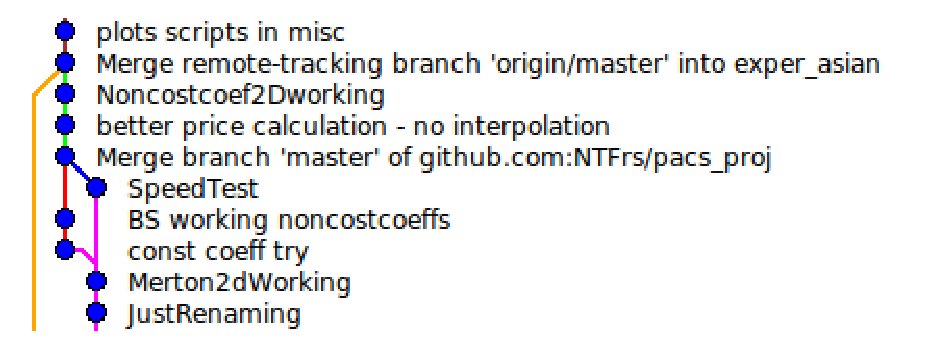
\includegraphics[width=\textwidth]{img/Git.eps}
 \caption{Cammino di alcuni \emph{branch} sui quali abbiamo lavorato. Immagine tratta da \textsf{gitk}}
 \label{fig:gitk}
\end{figure}

\section{\textsf{Doxygen}}
Infine, tutto il codice \`e commentato con il \emph{lexical-scanner} \textsf{Doxygen}, di molto facile utilizzo. 
%Cmake (molto comodo perch\'e abbiamo due piattaforme diverse ma funziona tutto perfettamente)\\Doxygen\\git (molto comodo per poterlo usare in 2)\\deal ii $\to$ utilit\`a offerte, pregi, difetti, come usarla, tutorial, eventualmente tutta la documentazione, gruppo molto attivo (abbiamo avuto una difficolt\`a ma l'abbiamo risolta subito)

\section{Profiler}
\paragraph{gprof}
Durante la scrittura dei codici finali, abbiamo trovato che alcune parti del programma era eccessivamente più lente rispetto a quando era stata fatta su file semplici. L'utilizzo del profiler \emph{gprof} ci ha permesso di analizzare e ristrutturare quella parte ottenendo uno speedup considerevole. In particolare, si trattava del calcolo dell'integrale con la trasformazione Price, e abbiamo scoperto che una delle funzioni di dealii di accesso a elementi della griglia era particolarmente lenta. Abbiamo risolto diminuendo quanto possibile il numero di chiamate ad essa.


\chapter{Codice}
\section{Introduzione}
In questo capitolo descriviamo come il problema \`e stato implementato da un punto di vista computazionale, elencando le varie classi scritte e le loro caratteristiche. Inizialmente mostriamo delle piccole classi che si occupano di gestire i parametri dei modelli e le loro densit\`a. Nella seconda sezione descriviamo gli oggetti opzione che costruiscono il sistema per risolvere il problema a elementi finiti in una e due dimensione. Questi oggetti utilizzano poi le funzioni di altri oggetti, \textsf{LevyIntegral}, per il calcolo della parte integrale. Successivamente, descriviamo brevemente la \emph{Factory} che abbiamo scritto per instanziare gli oggetti opzione e infine spieghiamo brevemente le linee guida per utilizzare questa libreria.
\section{Classi per i Modelli}
Il primo blocco di classi scritto nel nostro codice permette di gestire i vari modelli utilizzati per descrivere la dinamica del sottostante, in particolare i modelli di \emph{Blach\&Scholes}, \emph{Kou} e \emph{Merton}. Abbiamo quindi deciso di scrivere una classe astratta \textsf{Model}, che contenga i parametri comuni ai diversi oggetti e tutti i metodi utilizzati. Come possiamo osservare in figura \ref{modelbase}, da questa classe ereditano in maniera pubblica le tre classi modello non pi\`u astratte, ed esse contengono i parametri propri di ogni modello.
\begin{figure}[h!]
\begin{center}
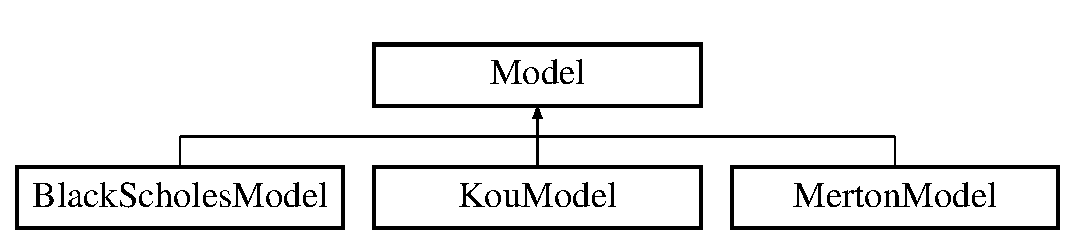
\includegraphics[width=12cm]{img/classModel.eps}
\caption{Gerarchia delle classi modello}
\end{center}
\label{modelbase}
\end{figure}
\section{Classi per Opzioni}
Le classi per Opzioni sono la componente centrale del programma e permettono di istanziare e gestire il problema di differenziale. Sono state scritte secondo le linee guida della libreria \textsf{deal.ii}. Le loro caratteristiche principali sono dunque le seguenti:
\begin{itemize}
\item {come tutte classi presentate nei \emph{tutorial} di \textsf{deal.ii}, anche le nostre classi hanno la dimensione (nel nostro caso 1 o 2) come parametro \textsf{template},}
\item {i pi\`u importanti metodi privati (o protetti) e pubblici dell'oggetto Opzione sono i seguenti:}
\begin{enumerate}
\item \textsf{virtual void setup\_system()};
\item \textsf{virtual void make\_grid()};
\item \textsf{virtual void assemble\_system()};
\item \textsf{virtual void refine\_grid()};
\item \textsf{virtual void setup\_integral()}, aggiunto da noi per allocare le classi che si occupano della parte integrale;
\item \textsf{virtual void solve()}, metodo che risolve il sistema lineare;
\item \textsf{virtual void run()}, metodo pubblico che chiama in ordine tutti i precedenti e calcola la soluzione.
\end{enumerate}
\end{itemize}
A questi metodi sono stati aggiunti altre funzioni che permettono di impostare alcune variabili del problema.\\Per quanto riguarda la struttura gerarchica di queste classi, poich\'e il nostro scopo \`e calcolare il prezzo di opzioni europee e americane con trasformazioni \emph{price} e \emph{logprice} e poich\'e alcuni metodi sono comuni ai diversi problemi e alle diverse trasformazioni, abbiamo deciso di sfruttare l'ereditariet\`a delle classi permessa dal c++ facendo chiamare al programma per ogni problema i metodi opportuni.
\begin{figure}[h!]
\begin{center}
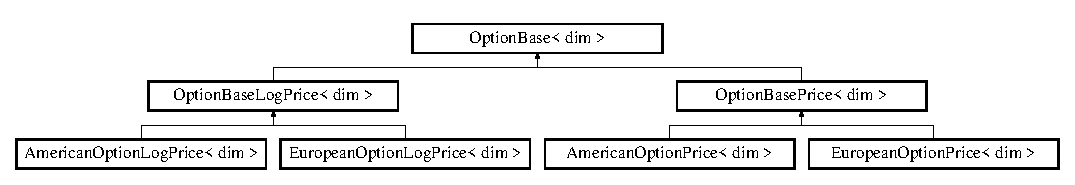
\includegraphics[width=12cm]{img/classOptionBase.eps}
\caption{Gerarchia delle classi opzione}
\end{center}
\label{optionbase}
\end{figure}
\subsection{\textsf{OptionBase$<$dim$>$}}
Entrando pi\`u nel dettaglio, come possiamo osservare nella figura \ref{optionbase}, abbiamo scritto una classe base \textsf{OptionBase$<$dim$>$} astratta, nel cui campo \textsf{protected} sono contenute tutte le variabili del problema, quali gli oggetti \textsf{dealii::FE\_Q$<$dim$>$}, \textsf{dealii::DoFHandler$<$dim$>$} e \textsf{dealii::Triangulation$<$dim$>$} che gestiscono elementi finiti, gradi di libert\`a e \emph{mesh}, gli oggetti che memorizzano le matrici e i \textsf{dealii::Vector$<$double$>$} della soluzione e del \emph{right hand side}. Per quanto riguarda l'oggetto che gestisce la matrice di sistema, poich\'e uno dei nostri problemi necessita di un \emph{solver} particolare non presente nella libreria utilizzata, ovvero il SOR, abbiamo deciso di scrivere un piccolo decoratore. Questo oggetto, \textsf{dealii::SparseMatrix\_PSOR$<$double, dim$>$} eredita pubblicamente da \textsf{dealii::SparseMatrix$<$double$>$} e aggiunge due metodi: uno che risolve il problema con l'ostacolo nel caso \emph{price} e uno nel caso \emph{logprice}. Come sappiamo, i costruttori non vengono ereditati, perci\`o sono stati riscritti in modo che chiamino i costruttori della classe base. Inoltre, siccome i metodi di \textsf{dealii::SparseMatrix$<$double$>$} non sono \textsf{virtual}, abbiamo aggiunto all'interno della nostra classe:
\begin{lstlisting}
// SparseMatrix methods
using dealii::SparseMatrix<number>::reinit;
using dealii::SparseMatrix<number>::add;
\end{lstlisting}
in modo che il compilatore capisca che deve utilizzare i metodi \textsf{reinit} e \textsf{add} di \textsf{dealii::SparseMatrix$<$double$>$}.\\\\Per quanto riguarda i costruttori di questa classe, essi sono specializzati per $1$ e $2$ dimensioni. In particolare, il costruttore $1$d prende un puntatore alla classe base \textsf{Model} e i vari parametri dell'opzione (quali tasso di interesse, scadenza e \emph{strike}), mentre il costruttore $2$d prende due puntatori a \textsf{Model} e i vari dati dell'opzione. I costruttori si occupano di creare gli oggetti relativi agli elementi finiti e li collegano alla \emph{mesh}. I metodi invece che implementiamo qui sono \textsf{void setup\_system()} che si occupa di creare lo \emph{sparsity pattern} delle matrici e inizializzarle e \textsf{void refine\_grid()} che esegue un adattamento della griglia.
\subsection{\textsf{OptionBasePrice$<$dim$>$} e \textsf{OptionBaseLogPrice$<$dim$>$}}
Le classi \textsf{OptionBasePrice$<$dim$>$} e \textsf{OptionBaseLogPrice$<$dim$>$}, anch'esse astratte, ereditano da \textsf{OptionBase$<$dim$>$} e definisco parte dei metodi descritti nell'introduzione. Le due classi implementano la funzione \textsf{void make\_grid()} che crea la \emph{mesh} nei casi \emph{price} e \emph{logprice}, ovvero con le opportune trasformazioni, il metodo \textsf{void assemble\_system()} che integra gli elementi finiti e costruisce le matrici di sistema in 1d e 2d e il metodo \textsf{double get\_price()}, che valuta la soluzione nel punto $\underline{x}=\underline{0}$ per il \emph{logprice} e $\underline{S}=(S_0^1, S_0^2)$ per il \emph{price}, ovvero che restituisce il prezzo dell'opzione. Infine, la classe \textsf{OptionBasePrice$<$dim$>$} implementa qui il metodo \textsf{void setup\_integral()} che istanzia dinamicamente un oggetto di tipo \textsf{LevyIntegral}, che si occupa di calcolare la parte integrale. \textsf{OptionBaseLogPrice$<$dim$>$} invece non lo istanzia qui ma nel "livello" di ereditarier\`a successivo poich\'e in questa trasformazione occorre conoscere le condizioni al bordo per poter calcolare l'integrale.
\subsection{\textsf{AmericanOption$<$dim$>$} e \textsf{EuropeanOption$<$dim$>$}}
Queste quattro classi alla base della piramide sono gli oggetti utilizzati per risolvere i vari problemi. Essi implementano le varie funzioni \textsf{void solve()} che risolvono il sistema lineare. In primo luogo quindi viene proiettata sulla \emph{mesh} la condizione finale (ovviamente diversa fra Put e Call, \emph{price} e \emph{logprice}) e successivamente parte il ciclo temporale che applica le condizioni al bordo, calcola il vettore integral $J$ se il modello non \`e \emph{Black\&Scholes} e risolve il sistema. Per quanto riguarda quest'ultimo passaggio, per l'europea abbiamo utilizzato un \emph{solver} utilizzato da \textsf{deal.ii}, ovvero \textsf{SparseDirectUMFPACK}, mentre per l'americana usiamo i \emph{solver} scritti all'interno del decoratore di \textsf{dealii::SparseMatrix$<$double$>$}.

%%%%%%%%%%%%%%%%%%%%%%%%%%%%%%%%%%%%%%%%%%%%%%%%%%%%%%%%%%%%%%%%%%%%%%
\section{Classi per il calcolo degli integrali}
Per il calcolo della parte integrale dell'equazione, ossia la quadratura di $\hat{\alpha}$ e il calcolo dei vettori $\mathbf{J}^i$ ad ogni iterazione temporale, sono state costruite una serie di classi. Tali classi ereditano da una classe comune di base che definisce l'interfaccia. Usando questo schema con ereditarietà (che si può vedere in figura \ref{fig:levybase}) si riesce a mantenere un interfaccia comune, e permette di allocare classi specifiche per modelli specifici. Cosi come le classi opzione, anche queste sono classi templatizzate sulla dimensione, poiché il calcolo dell'integrale può essere anche molto diverso fra una dimensione e l'altra.
\begin{figure}[h!]
\begin{center}
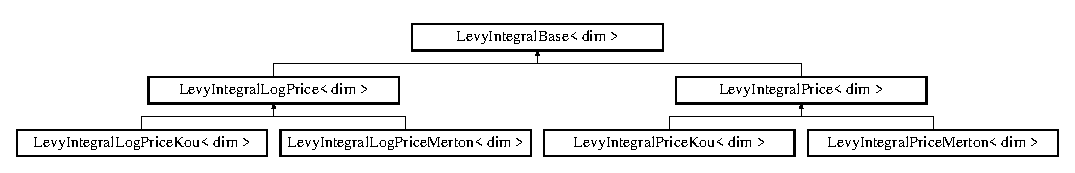
\includegraphics[width=12cm]{img/classLevyIntegralBase.eps}
\label{fig:levybase}
\end{center}
\end{figure}
\subsection{La classe base \textsf{LevyIntegralBase}}
Questa classe astratta serve per definire un interfaccia che tutte le classi per la quadratura dell'integrale dovrebbero sfruttare. Inoltre a implementa alcuni metodi di base che possono essere utili alle classi figlie.\\
I due metodi \emph{core} della classe sono \textsf{compute\_alpha()}, che calcola il valore degli $\hat{\alpha}^i$, e \textsf{compute\_J()}, che calcola il valore della parte integrale da usare nel \emph{rhs}. È interessante notare che questa classe base definisce già una funzione che calcola $\hat{\alpha}^i$ generica, ossia con una quadratura composita con nodi di Gauss, e che funziona dunque con qualsiasi modello.

\subsection{Le classi \textsf{LevyIntegralPrice} e \textsf{LevyIntegralLogPrice}}
La seconda parte dell'integrale, i vettori $\mathbf{J}^i$ è totalmente diversa a seconda che si utilizzi la forma Price o la forma LogPrice. Per questo vi sono queste due classi che ereditano da \textsf{LevyIntegralBase}. Siccome sono ancora generiche e non per un modello specifico, ereditano da quest'ultima il metodo \textsf{compute\_alpha()}. Inoltre queste funzionano con un modello qualunque.

\paragraph{\textsf{LevyIntegralLogPrice}}
Questa classe implementa \textsf{compute\_J()} per la forma logprice, ed è sostanzialmente più semplice, ma anche più lenta rispetto a price.\\
In sostanza, sia in una che in due dimensioni (e potenzialmente in più), il calcolo di $\mathbf{J}^i$ viene svolto facendo un ciclo su tutti i nodi della griglia e in ciascuno calcolando il valore dell'integrale in quel punto e per fare ciò fa ricorso alla classe ausiliaria \textsf{Solution\_Trimmer}. Tale classe è praticamente un funtore che, inizializzato con la soluzione e la mappatura dei gradi di libertà di Deal.II (il \textsf{DoFHandler}) agisce diversamente a seconda che il punto stia dentro o fuori dal dominio. Nel primo caso chiama una funzione di Deal.II che individua in che cella si trova il nodo e restituisce il valore della funzione in tale punto, nel secondo caso impone il valore al bordo. La parte computazionalmente costosa è appunto la valutazione in un punto interno al dominio, poiché deve individuare in quale cella si trova (ricordiamo qui che la funzione incognita va valutata nel punto $y_l+x_i$, dove $y_l$ sono i nodi di quadratura e $x_i$ il nodo attuale, quindi ad ogni nodo in punti diversi).\\
Una volta ottenuto il valore della soluzione nel punto (sia esso dentro o fuori dal dominio) è possibile effettuare la quadratura dell'integrale. A questo livello, utilizza una quadratura generica poiché non vi è un modello specifico.
\paragraph{\textsf{LevyIntegralPrice}}
\label{subsec:LevyIntegralPrice}
Questa classe implementa \textsf{compute\_J()} specializzando il metodo sul parametro template, ossia la dimensione. Infatti, come già spiegato nella sezione \ref{sec:Price}, il modo in cui calcolare $\mathbf{J}^i$ è fondamentalmente diverso.\\
In una dimensione, per ogni nodo della griglia, bisogna integrare sulla stessa griglia, e quindi si scorrono tutte le celle calcolando il contributo. In due dimensioni, il contributo a $\mathbf{J}^1$ nel nodo $S_i$ è calcolato sulla retta monodimensionale parallela all'asse delle ascisse, mentre il contributo a $\mathbf{J}^2$ è calcolato lungo la retta parallela all'asse delle ordinate. Quindi si scorrono le facce delle celle della griglia, e su ciascuna faccia si calcola il contributo a ogni nodo appartenente alla retta su cui giace la faccia in questione. Sebbene è una procedura complicata \todo{richiede una griglia strutturata?} e richiede che tutti i nodi vengano visitati ma solo alcuni usati per la faccia corrente, è più rapida rispetto al calcolo con il metodo logprice. Infatti, in questo caso la funzione va valutata nei nodi di quadratura che cadono sulla faccia attuale, quindi dalla posizione nota.

\subsection{Le classi figlie per modelli specifici}

Come si nota in figura \ref{fig:levybase}, esistono poi delle classi derivate da \textsf{LevyIntegralPrice} e \textsf{LevyIntegralLogPrice}. Esse implementano di nuovo i metodi per il calcolo delle parti integrali con dei nodi di quadratura specifici ai modelli. In particolare \textsf{LevyIntegralPriceKou} e \textsf{LevyIntegralLogPriceKou} utilizzano nodi di Gauss-Laguerre, mentr \textsf{LevyIntegralPriceMerton} e \textsf{LevyIntegralLogPriceMerton} utilizzano nodi di Gauss-Hermite. Le due classi ereditate da \textsf{LevyIntegralPrice} reimplementano solo la parte relativa ad $\hat{\alpha}^i$, poiché la parte $\mathbf{J}$ rimane uguale.\\

Nel caso si vogliano aggiungere alla libreria alri modelli, questo design permette di creare nuove classi specifiche per l'integrale che ereditano dal secondo livello, dovendo modificare solo una piccola parte.

\section{\emph{Factory}}
Data la complessit\`a strutturale delle classi Opzioni, abbiamo deciso di scrivere utilizzare il \emph{design pattern} della \emph{factory}, altrimenti noto come costruttore virtuale, per permettere a un qualsiasi utente di istanziare l'oggetto giusto per il suo problema. Abbiamo quindi creato una classe, \textsf{OptionFactory} che ha costruttore di default, costruttore di copia e operatore di copia privati, perci\`o non \`e possibile istanziare la classe, e abbiamo scritto il seguente metodo:
\begin{lstlisting}
static OptionFactory * instance()
        {
                static OptionFactory instance;
                return &instance;
        }
\end{lstlisting}
Questa funzione permette di istanziare uno e un solo oggetto della classe \textsf{OptionFactory}, che \`e quindi un \emph{singleton}. Oltre a questo metodo, abbiamo due funzioni \textsf{std::unique\_ptr$<$OptionBase$<$dim$>$ $>$ create(...)} con il parametro \textsf{dim} specializzato su una e due dimensioni che prendono come argomenti il tipo di opzione, europea o americana, put o call, il tipo di trasformazione, i modelli dei sottostanti e i vari parametri dell'opzione.
\section{Come utilizzare la libreria}

\chapter{Risultati}
\chapter{Estensioni}
Il programma che abbiamo scritto si presta molto a possibili estensioni, su molti livelli. In particolare, a partire dalle classi base \textsf{OptionBasePrice$<$dim$>$} e \textsf{OptionBaseLogPrice$<$dim$>$} \`e possibile scrivere dei \emph{solver} che prezzino tutte le opzioni barriera, ovvero opzioni caratterizzate da condizioni al bordi di \emph{Dirichlet} nulle in alcune parti o su tutto il bordo dominio.\\\`E inoltre possibile estendere la libreria in modo che prezzi opzioni con altri modelli, per esempio ad attivit\`a infinita, caratterizzati cio\`e da misure di L\'evy non limitate (come, ad esempio, il \emph{Normal Inverse Gaussian} e il \emph{Variance Gamma}). Per fare ci\`o occorre modificare le classi integrale, in modo che calcolino il parametro $\lambda$, che per questi modelli \`e incognito e calcolare all'interno della classe opzione la diffusione che approssima i piccoli salti (che in questo caso, sono infiniti).\\Un'altra estensione possibile, ma abbastanza delicata, \`e estendere il programma al calcolo di opzioni con tre sottostanti, ovvero risolvere un PIDE 3d. Teoricamente l'equazione sarebbe formalmente la stessa, con l'aggiunta di un terzo integrale su $\mathbb{R}$. Occorrerebbe tuttavia prestare attenzione a dove integrare i vari integrali: in 2d, infatti, abbiamo calcolato gli integrali sui lati dei quadrilateri che costituiscono la \emph{mesh}, in 3d si dovrebbe invece integrare sui lati delle facce dei parallelepipedi????\\Si potrebbe provare poi a utilizzare le funzioni offerte dalla libreria \textsf{deal.ii} per la soluzione del problema con memoria distribuita. Per quanto riguarda la parte PDE si pu\`o sfruttare quanto implementato nella libreria, mentre per il calcolo dell'integrale in \emph{price} occorrerebbe spedire tutta la soluzione a tutti i processi (perch\'e il termine \`e non locale), in \emph{log-price} invece tutti i processi devono conoscere tutta la griglia, per poter valutare la funzione nei punti $y+x$ (\ref{intnonlocal}).\\\\
Heston?
%Aggiungere altri modelli (NIG, VG), provare altre opzioni, farlo in 3d, Heston?, memoria distribuita.
\clearpage
\addcontentsline{toc}{chapter}{Bibliografia}
%stile della bibliografia
\bibliographystyle{plain}
%questo specifica il file da usare
\bibliography{Fonti}

\iffalse
\begin{thebibliography}{9}
\bibitem{} R Cont, P Tankov. \emph{Financial Modelling with Jump Processes}. Chapman \& Hall, 2004.
\bibitem{} R Seydel. \emph{Tools for Computational Finance}. Springer, 2009.
\bibitem{} Y Achdou, O Pironneau. \emph{Computational Methods for Option Pricing}. SIAM, 2005.
\bibitem{} J Tao, L Xin, Y Zhengzhou. \emph{Finite Element Algorithms for Pricing 2-D Basket Options}. 2009.
\bibitem{} Z Jinghui. \emph{Multi-Asset Option Pricing with L\'evy process}. 2009.
\bibitem{} A Quarteroni. \emph{Modellistica numerica per problemi differenziali}. Springer, 2008.
\bibitem{} A Quarteroni, R Sacco, F Saleri. \emph{Matematica Numerica}. Springer, 2008.
\bibitem{} L Feng, V Linetsky, J L Morales, J Nocedal. \emph{On the Solution of Complementarity Problems Arising in American Options Pricing}. 2010.
\bibitem{} E Gamma, R Helm, R Johnson, V Vlissides. \emph{Design Patterns}. 1997.

\end{thebibliography}
\fi
\end{document}
